%% bare_conf.tex
%% V1.4
%% 2012/12/27
%% by Michael Shell
%% See:
%% http://www.michaelshell.org/
%% for current contact information.
%%
%% This is a skeleton file demonstrating the use of IEEEtran.cls
%% (requires IEEEtran.cls version 1.8 or later) with an IEEE conference paper.
%%
%% Support sites:
%% http://www.michaelshell.org/tex/ieeetran/
%% http://www.ctan.org/tex-archive/macros/latex/contrib/IEEEtran/
%% and
%% http://www.ieee.org/

%%*************************************************************************
%% Legal Notice:
%% This code is offered as-is without any warranty either expressed or
%% implied; without even the implied warranty of MERCHANTABILITY or
%% FITNESS FOR A PARTICULAR PURPOSE! 
%% User assumes all risk.
%% In no event shall IEEE or any contributor to this code be liable for
%% any damages or losses, including, but not limited to, incidental,
%% consequential, or any other damages, resulting from the use or misuse
%% of any information contained here.
%%
%% All comments are the opinions of their respective authors and are not
%% necessarily endorsed by the IEEE.
%%
%% This work is distributed under the LaTeX Project Public License (LPPL)
%% ( http://www.latex-project.org/ ) version 1.3, and may be freely used,
%% distributed and modified. A copy of the LPPL, version 1.3, is included
%% in the base LaTeX documentation of all distributions of LaTeX released
%% 2003/12/01 or later.
%% Retain all contribution notices and credits.
%% ** Modified files should be clearly indicated as such, including  **
%% ** renaming them and changing author support contact information. **
%%
%% File list of work: IEEEtran.cls, IEEEtran_HOWTO.pdf, bare_adv.tex,
%%                    bare_conf.tex, bare_jrnl.tex, bare_jrnl_compsoc.tex,
%%                    bare_jrnl_transmag.tex
%%*************************************************************************

% *** Authors should verify (and, if needed, correct) their LaTeX system  ***
% *** with the testflow diagnostic prior to trusting their LaTeX platform ***
% *** with production work. IEEE's font choices can trigger bugs that do  ***
% *** not appear when using other class files.                            ***
% The testflow support page is at:
% http://www.michaelshell.org/tex/testflow/



% Note that the a4paper option is mainly intended so that authors in
% countries using A4 can easily print to A4 and see how their papers will
% look in print - the typesetting of the document will not typically be
% affected with changes in paper size (but the bottom and side margins will).
% Use the testflow package mentioned above to verify correct handling of
% both paper sizes by the user's LaTeX system.
%
% Also note that the "draftcls" or "draftclsnofoot", not "draft", option
% should be used if it is desired that the figures are to be displayed in
% draft mode.
%
\documentclass[conference]{IEEEtran}
% Add the compsoc option for Computer Society conferences.
%
% If IEEEtran.cls has not been installed into the LaTeX system files,
% manually specify the path to it like:
% \documentclass[conference]{../sty/IEEEtran}

%\setcounter{secnumdepth}{5}
%\setcounter{tocdepth}{5}



% Some very useful LaTeX packages include:
% (uncomment the ones you want to load)


% For directly writing german umlauts uncomment the appropriate line for
% your operating system:
% Windows:
 \usepackage[ansinew]{inputenc}
% Linux:
%\usepackage[latin1]{inputenc}
% Mac
% \usepackage[applemac]{inputenc}
% If none of the above lines work you can also try the following:
% \usepackage[utf8]{inputenc}



% *** MISC UTILITY PACKAGES ***
%
%\usepackage{ifpdf}
% Heiko Oberdiek's ifpdf.sty is very useful if you need conditional
% compilation based on whether the output is pdf or dvi.
% usage:
% \ifpdf
%   % pdf code
% \else
%   % dvi code
% \fi
% The latest version of ifpdf.sty can be obtained from:
% http://www.ctan.org/tex-archive/macros/latex/contrib/oberdiek/
% Also, note that IEEEtran.cls V1.7 and later provides a builtin
% \ifCLASSINFOpdf conditional that works the same way.
% When switching from latex to pdflatex and vice-versa, the compiler may
% have to be run twice to clear warning/error messages.






% *** CITATION PACKAGES ***
%
%\usepackage{cite}
% cite.sty was written by Donald Arseneau
% V1.6 and later of IEEEtran pre-defines the format of the cite.sty package
% \cite{} output to follow that of IEEE. Loading the cite package will
% result in citation numbers being automatically sorted and properly
% "compressed/ranged". e.g., [1], [9], [2], [7], [5], [6] without using
% cite.sty will become [1], [2], [5]--[7], [9] using cite.sty. cite.sty's
% \cite will automatically add leading space, if needed. Use cite.sty's
% noadjust option (cite.sty V3.8 and later) if you want to turn this off
% such as if a citation ever needs to be enclosed in parenthesis.
% cite.sty is already installed on most LaTeX systems. Be sure and use
% version 4.0 (2003-05-27) and later if using hyperref.sty. cite.sty does
% not currently provide for hyperlinked citations.
% The latest version can be obtained at:
% http://www.ctan.org/tex-archive/macros/latex/contrib/cite/
% The documentation is contained in the cite.sty file itself.






% *** GRAPHICS RELATED PACKAGES ***
%
\ifCLASSINFOpdf
  \usepackage[pdftex]{graphicx}
  % declare the path(s) where your graphic files are
  % \graphicspath{{../pdf/}{../jpeg/}}
  % and their extensions so you won't have to specify these with
  % every instance of \includegraphics
  % \DeclareGraphicsExtensions{.pdf,.jpeg,.png}
\else
  % or other class option (dvipsone, dvipdf, if not using dvips). graphicx
  % will default to the driver specified in the system graphics.cfg if no
  % driver is specified.
  \usepackage[dvips]{graphicx}
  % declare the path(s) where your graphic files are
  % \graphicspath{{../eps/}}
  % and their extensions so you won't have to specify these with
  % every instance of \includegraphics
  % \DeclareGraphicsExtensions{.eps}
\fi
% graphicx was written by David Carlisle and Sebastian Rahtz. It is
% required if you want graphics, photos, etc. graphicx.sty is already
% installed on most LaTeX systems. The latest version and documentation
% can be obtained at: 
% http://www.ctan.org/tex-archive/macros/latex/required/graphics/
% Another good source of documentation is "Using Imported Graphics in
% LaTeX2e" by Keith Reckdahl which can be found at:
% http://www.ctan.org/tex-archive/info/epslatex/
%
% latex, and pdflatex in dvi mode, support graphics in encapsulated
% postscript (.eps) format. pdflatex in pdf mode supports graphics
% in .pdf, .jpeg, .png and .mps (metapost) formats. Users should ensure
% that all non-photo figures use a vector format (.eps, .pdf, .mps) and
% not a bitmapped formats (.jpeg, .png). IEEE frowns on bitmapped formats
% which can result in "jaggedy"/blurry rendering of lines and letters as
% well as large increases in file sizes.
%
% You can find documentation about the pdfTeX application at:
% http://www.tug.org/applications/pdftex





% *** MATH PACKAGES ***
%
\usepackage[cmex10]{amsmath}
\usepackage{amsfonts}
% A popular package from the American Mathematical Society that provides
% many useful and powerful commands for dealing with mathematics. If using
% it, be sure to load this package with the cmex10 option to ensure that
% only type 1 fonts will utilized at all point sizes. Without this option,
% it is possible that some math symbols, particularly those within
% footnotes, will be rendered in bitmap form which will result in a
% document that can not be IEEE Xplore compliant!
%
% Also, note that the amsmath package sets \interdisplaylinepenalty to 10000
% thus preventing page breaks from occurring within multiline equations. Use:
%\interdisplaylinepenalty=2500
% after loading amsmath to restore such page breaks as IEEEtran.cls normally
% does. amsmath.sty is already installed on most LaTeX systems. The latest
% version and documentation can be obtained at:
% http://www.ctan.org/tex-archive/macros/latex/required/amslatex/math/





% *** SPECIALIZED LIST PACKAGES ***
%
%\usepackage{algorithmic}
% algorithmic.sty was written by Peter Williams and Rogerio Brito.
% This package provides an algorithmic environment fo describing algorithms.
% You can use the algorithmic environment in-text or within a figure
% environment to provide for a floating algorithm. Do NOT use the algorithm
% floating environment provided by algorithm.sty (by the same authors) or
% algorithm2e.sty (by Christophe Fiorio) as IEEE does not use dedicated
% algorithm float types and packages that provide these will not provide
% correct IEEE style captions. The latest version and documentation of
% algorithmic.sty can be obtained at:
% http://www.ctan.org/tex-archive/macros/latex/contrib/algorithms/
% There is also a support site at:
% http://algorithms.berlios.de/index.html
% Also of interest may be the (relatively newer and more customizable)
% algorithmicx.sty package by Szasz Janos:
% http://www.ctan.org/tex-archive/macros/latex/contrib/algorithmicx/




% *** ALIGNMENT PACKAGES ***
%
%\usepackage{array}
% Frank Mittelbach's and David Carlisle's array.sty patches and improves
% the standard LaTeX2e array and tabular environments to provide better
% appearance and additional user controls. As the default LaTeX2e table
% generation code is lacking to the point of almost being broken with
% respect to the quality of the end results, all users are strongly
% advised to use an enhanced (at the very least that provided by array.sty)
% set of table tools. array.sty is already installed on most systems. The
% latest version and documentation can be obtained at:
% http://www.ctan.org/tex-archive/macros/latex/required/tools/


% IEEEtran contains the IEEEeqnarray family of commands that can be used to
% generate multiline equations as well as matrices, tables, etc., of high
% quality.




% *** SUBFIGURE PACKAGES ***
%\ifCLASSOPTIONcompsoc
%  \usepackage[caption=false,font=normalsize,labelfont=sf,textfont=sf]{subfig}
%\else
%  \usepackage[caption=false,font=footnotesize]{subfig}
%\fi
% subfig.sty, written by Steven Douglas Cochran, is the modern replacement
% for subfigure.sty, the latter of which is no longer maintained and is
% incompatible with some LaTeX packages including fixltx2e. However,
% subfig.sty requires and automatically loads Axel Sommerfeldt's caption.sty
% which will override IEEEtran.cls' handling of captions and this will result
% in non-IEEE style figure/table captions. To prevent this problem, be sure
% and invoke subfig.sty's "caption=false" package option (available since
% subfig.sty version 1.3, 2005/06/28) as this is will preserve IEEEtran.cls
% handling of captions.
% Note that the Computer Society format requires a larger sans serif font
% than the serif footnote size font used in traditional IEEE formatting
% and thus the need to invoke different subfig.sty package options depending
% on whether compsoc mode has been enabled.
%
% The latest version and documentation of subfig.sty can be obtained at:
% http://www.ctan.org/tex-archive/macros/latex/contrib/subfig/




% *** FLOAT PACKAGES ***
%
%\usepackage{fixltx2e}
% fixltx2e, the successor to the earlier fix2col.sty, was written by
% Frank Mittelbach and David Carlisle. This package corrects a few problems
% in the LaTeX2e kernel, the most notable of which is that in current
% LaTeX2e releases, the ordering of single and double column floats is not
% guaranteed to be preserved. Thus, an unpatched LaTeX2e can allow a
% single column figure to be placed prior to an earlier double column
% figure. The latest version and documentation can be found at:
% http://www.ctan.org/tex-archive/macros/latex/base/


%\usepackage{stfloats}
% stfloats.sty was written by Sigitas Tolusis. This package gives LaTeX2e
% the ability to do double column floats at the bottom of the page as well
% as the top. (e.g., "\begin{figure*}[!b]" is not normally possible in
% LaTeX2e). It also provides a command:
%\fnbelowfloat
% to enable the placement of footnotes below bottom floats (the standard
% LaTeX2e kernel puts them above bottom floats). This is an invasive package
% which rewrites many portions of the LaTeX2e float routines. It may not work
% with other packages that modify the LaTeX2e float routines. The latest
% version and documentation can be obtained at:
% http://www.ctan.org/tex-archive/macros/latex/contrib/sttools/
% Do not use the stfloats baselinefloat ability as IEEE does not allow
% \baselineskip to stretch. Authors submitting work to the IEEE should note
% that IEEE rarely uses double column equations and that authors should try
% to avoid such use. Do not be tempted to use the cuted.sty or midfloat.sty
% packages (also by Sigitas Tolusis) as IEEE does not format its papers in
% such ways.
% Do not attempt to use stfloats with fixltx2e as they are incompatible.
% Instead, use Morten Hogholm'a dblfloatfix which combines the features
% of both fixltx2e and stfloats:
%
% \usepackage{dblfloatfix}
% The latest version can be found at:
% http://www.ctan.org/tex-archive/macros/latex/contrib/dblfloatfix/




% *** PDF, URL AND HYPERLINK PACKAGES ***
%
%\usepackage{url}
% url.sty was written by Donald Arseneau. It provides better support for
% handling and breaking URLs. url.sty is already installed on most LaTeX
% systems. The latest version and documentation can be obtained at:
% http://www.ctan.org/tex-archive/macros/latex/contrib/url/
% Basically, \url{my_url_here}.




% *** Do not adjust lengths that control margins, column widths, etc. ***
% *** Do not use packages that alter fonts (such as pslatex).         ***
% There should be no need to do such things with IEEEtran.cls V1.6 and later.
% (Unless specifically asked to do so by the journal or conference you plan
% to submit to, of course. )


% add custom packages
\usepackage{color}
\definecolor{tumblue}{rgb}{0, 0.4, 0.74}



% correct bad hyphenation here
\hyphenation{op-tical net-works semi-conduc-tor}

\usepackage[font=scriptsize,labelfont=bf,labelformat=empty,justification=centering]{caption}
\usepackage{listings} 



\begin{document}

% Add the seminar's cover page
\begin{figure*}[!h]

  
\includegraphics{./images/IN.pdf} \hfill 
\includegraphics{./images/tumlogo.pdf}
 
  \vspace*{1cm}
  {\large \textsf{Fakult{\"a}t f{\"u}r Informatik}}\\
  {\large \textsf{Lehrstuhl f{\"u}r Echtzeitsysteme und Robotik}}\\
   

  \vspace*{5cm}
%
%
% TITEL DER ARBEIT
%
%
  {\color{tumblue} \Huge \bf \textsf{Get Me Out Of Here: \\\\Determing Optimal Policies}}\\  % HIER EINSETZEN!

  \vspace*{1cm}
%
%
% NAME DES STUDENTEN (auf Titelblatt)
%
% 
  {\Large \bf \textsf{Marcel Bruckner}}\\   % HIER EINSETZEN!
 
  \vspace*{8cm}
  {\Large \textsf{Seminar \emph{Cyber-Physical Systems} WS 2017/18}}\\
 
  \vspace*{1cm} 
  \begin{tabular}{ll}
%
%
% NAME DES BETREUERS
%
%
    {\Large \bf \textsf{Advisor:}} &
    {\Large \textsf{Christian Pek}}\\                  % HIER EINSETZEN!
    \\

    {\Large \bf \textsf{Supervisor:}} &
    {\Large \textsf{Prof.~Dr.-Ing. Matthias Althoff}}\\
    \\

%
%
% ABGABETERMIN
%
%
    {\Large \bf \textsf{Submission:}} &
    {\Large \textsf{07. February 2018}}

  \end{tabular}
  
\end{figure*}


%
% paper title
% can use linebreaks \\ within to get better formatting as desired
% Do not put math or special symbols in the title.
\title{Get Me Out Of Here: Determining Optimal Policies}


% author names and affiliations
% use a multiple column layout for up to three different
% affiliations
\author{\IEEEauthorblockN{Marcel Bruckner}
\IEEEauthorblockA{Technische Universit\"at M\"unchen\\
Email: mbruckner94@gmail.com}}

% conference papers do not typically use \thanks and this command
% is locked out in conference mode. If really needed, such as for
% the acknowledgment of grants, issue a \IEEEoverridecommandlockouts
% after \documentclass

% use for special paper notices
%\IEEEspecialpapernotice{(Invited Paper)}



% make the title area
\maketitle

% As a general rule, do not put math, special symbols or citations
% in the abstract
\begin{abstract}
This paper gives a brief overview on the field of dynamic programming and it's applicability in robot motion planning. Exemplary, some use cases in other papers will be shown and an algorithm to find optimal policies in a maze will be introduced.
\end{abstract}

% no keywords




% For peer review papers, you can put extra information on the cover
% page as needed:
% \ifCLASSOPTIONpeerreview
% \begin{center} \bfseries EDICS Category: 3-BBND \end{center}
% \fi
%
% For peerreview papers, this IEEEtran command inserts a page break and
% creates the second title. It will be ignored for other modes.
\IEEEpeerreviewmaketitle

\section{Introduction}
Remember the game Labyrinth, in which the game represents a maze where the field is build up by fixed and moving pieces showing walls and passages. The goal of the game is to rearrange the maze by moving rows of not fixed tiles and enable ones game character to find treasures and return them to goal tiles.
\\
To reach the goal in this game, a way for calculating the shortest path to exit the maze has to be found. This can be achieved with classical motion planning algorithms, like Dijkstras Algorithm or Breadth-First Search, but also with \textbf{Dynamic Programming}, which will be used in this Paper.
\\
Therefore, let a grid map $M=\mathbb{N}^{n \times m}$ containing static walls $M(i,j)=\infty$ represent the maze and let there be a set of exits $X_\text{goal}$ in the labyrinth which the player wants to reach.
\\
The goal of this paper is to point out ways to determine optimal policies $P=\mathbb{N}^{nxm}\rightarrow A$ to exit the labyrinth. To achieve this, a way to calculate the value $v(i,j)$ of the current position is introduced from what the actual best action can be derived.\\
Later on, the algorithm will look like in the following example:


\begin{figure}[h]
\centering
\begin{minipage}[t]{0.3\linewidth}
\centering
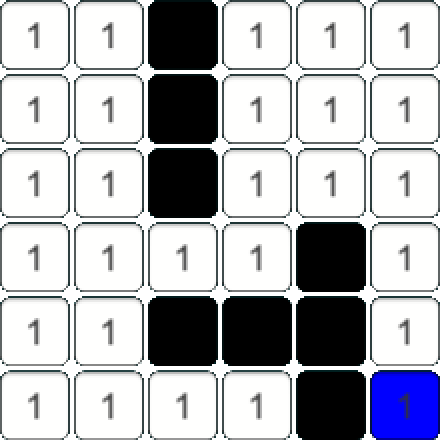
\includegraphics[width=1\textwidth]{images/intro/original.png}
\caption{The original grid showing the cost of each tile, walls (black) and goals (blue).}
\end{minipage}
\hfill
\begin{minipage}[t]{0.3\linewidth}
\centering
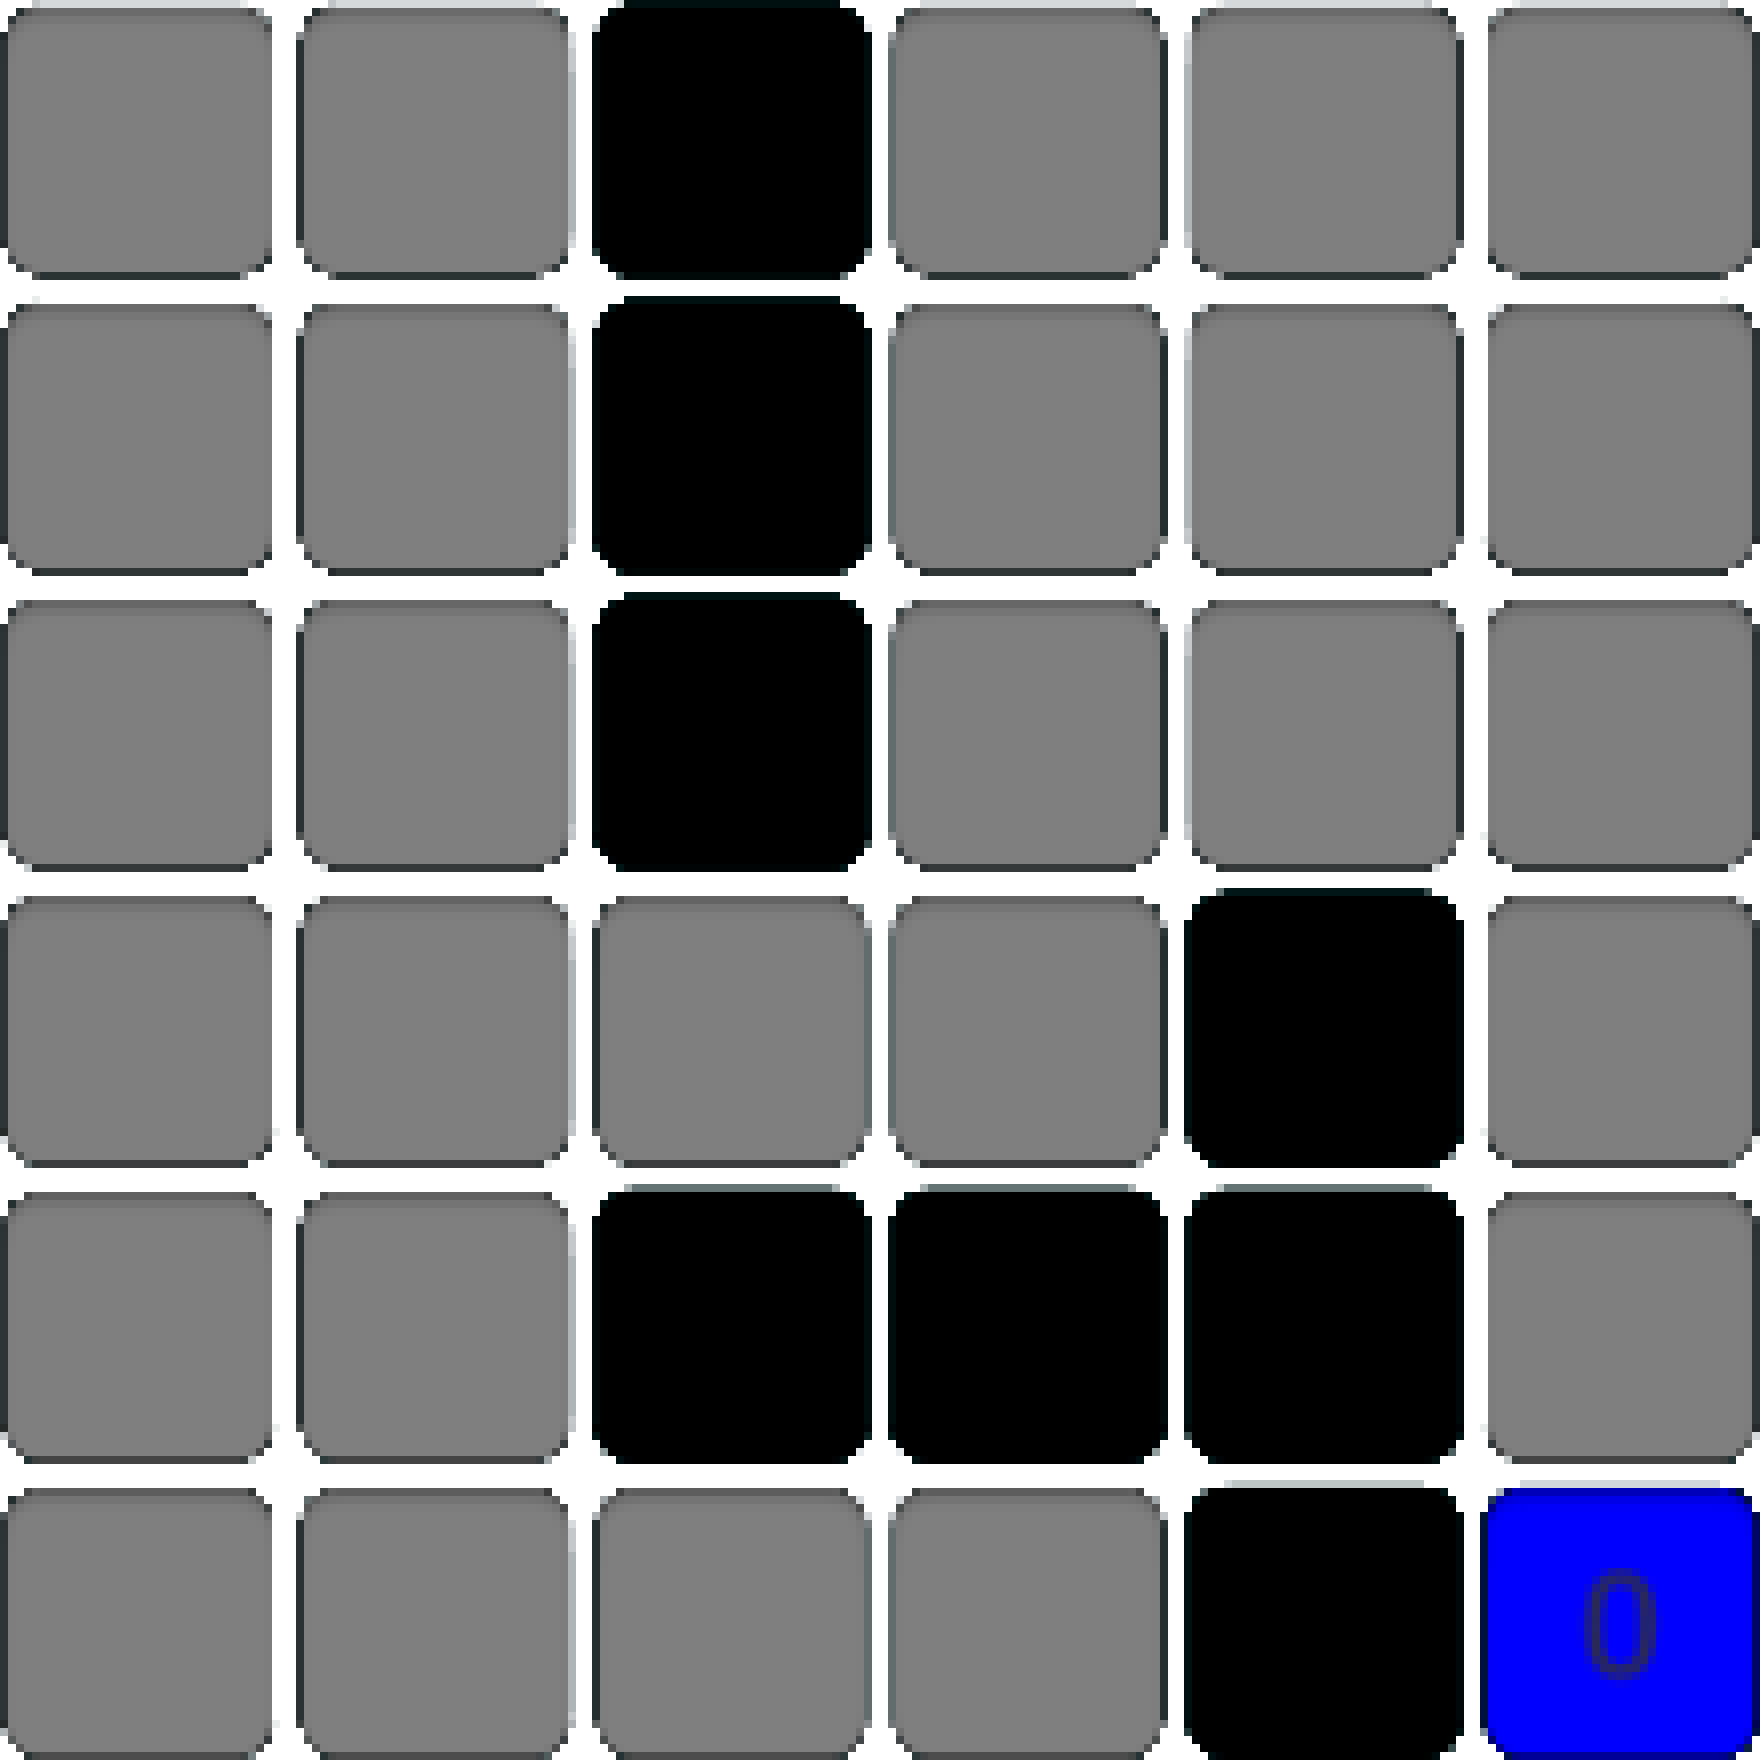
\includegraphics[width=1\textwidth]{images/intro/init.png}
\caption{Initialization of the algorithm with $\infty$ cost. Only the goal (blue) is set and is the starting point. It has a value of 0.}
\end{minipage}
\hfill
\begin{minipage}[t]{0.3\linewidth}
\centering
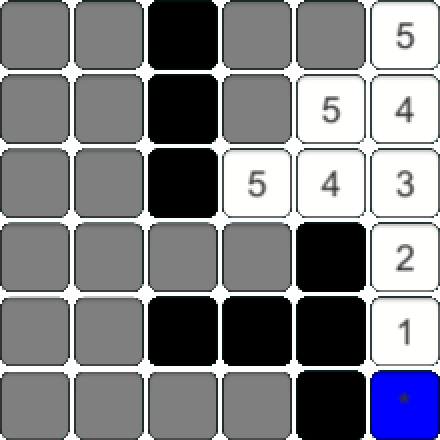
\includegraphics[width=1\textwidth]{images/intro/few.png}
\caption{After a few iterations the values of some tiles are set. The value is equal to the length of the shortest path to the goal.}
\end{minipage}


\begin{minipage}[t]{0.3\linewidth}
\centering
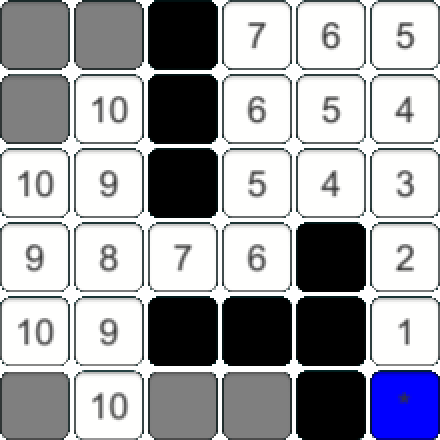
\includegraphics[width=1\textwidth]{images/intro/more.png}
\caption{A few more iterations. The algorithm is reaching tiles further away from the goal.}
\end{minipage}
\hfill
\begin{minipage}[t]{0.3\linewidth}
\centering
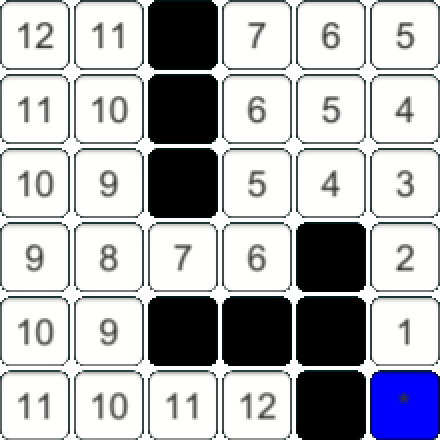
\includegraphics[width=1\textwidth]{images/intro/final.png}
\caption{All values are calculated. Every tile is holding its value.}
\end{minipage}
\hfill
\begin{minipage}[t]{0.3\linewidth}
\centering
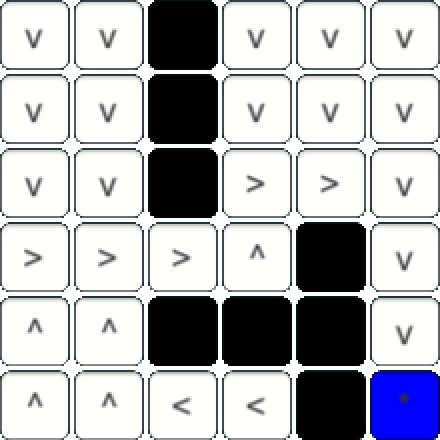
\includegraphics[width=1\textwidth]{images/intro/policy.png}
\caption{The final optimal policy showing the best action for every position derived from the values of the tiles.}
\end{minipage}
\end{figure}


\section{Fundamentals}
\subsection{What is Dynamic Programming}
Dynamic Programming is a method used in mathematical optimization and computer programming that transforms complex problems into sequences of simpler subproblems. Each of those subproblems will be solved just once and their solutions will be stored, so when reoccuring, the previously computed solution will be looked up to save computation time.
\\
For solving a problem with Dynamic Programming, the problem gets broken down and by recursively finding the optimal solution for the subproblems a optimal solution for the whole problem can be found.
\\
It provides a general framework for analyzing many problem types, like the planning of industrial production lines, scheduling of patients at a medical clinic, long term investment programs and, of course, robot motion planning.
\\
Underlying of these problems is always a sequence of decisions that have to be made within a finite number of stages. E.g. a robot wants to move from one position to another by a finite number of steps and investment programs do have to calculate their wealth at every step in time.\\
A sequential decision making problem with finite stages can be defined with the following statements:
\begin{itemize}
\item $\mathbf{X}$ is the set of all possible states of the system;
\item $\mathbf{U}$ is the set of controls or also called transformations;
\item $\mathbf{f}: X \times U \mapsto X$ is a transition function, a mapping specifying the next state $f(x,u)$ if control $u$ is executed when the system is in state $x$;
\item $\mathbf{c}: X \times U \mapsto \mathbb{R}$ is a cost function that gives a real value $c(x, u)$ obtained if control $u$ is executed when the system is in the state $x$;
\item $\mathbf{v}: X \mapsto \mathbb{R}$ is a value function that gives a real value $v(x)$ associated with the state $x$;
\item $\mathbf{x_\text{init}} \in X$ is the initial state of the system. \cite{OktayArslan.December2015}
\end{itemize}

%---------------------------------
%\\
%Underlying of these problems is always a multistage decision problem. "The characteristic feature of these problems is that they concern a system whose state $x_k \in X_k$ evolves according to a recursive relation of the form
%\begin{equation*}
%x_{k+1} = f_k(x_k, a_k, w_k); \quad k = 0,1,...
%\end{equation*}
%where $a_k \in C_k$ is the decision in period $k$ and $w_k \in D_k$ is the value in period $k$"\cite{Pra.1995}.
\subsection{Richard Bellman}
Dynamic Programming was introduced by the american mathematician Richard Bellman who was working on multistage decision problems from 1949 until 1955. After he received his Ph.D. from Princeton at the age of 25, he started his research at RAND Corporation (Research and Development), where his secretary really had a hatred of the term \textit{mathematical research}. So he started his work with finding a name under which he could hide his projects.
\\
He was interested in planning, decision making and thinking, but none of these were good terms, so he decided on the word programming, and because of his love for physics and his ideas in multistage and time varying problems, he came to the conclusion that dynamic is the best adjective to accompany it.\\
Following the name Dynamic Programming was born and no one could imagine what he was doing which made it perfect for hiding his mathematical research. \cite{Dreyfus.2002}
\subsection{The Principle of Optimality}
For starting a more precise discussion, let define the term optimal policy:
\begin{itemize}
\item A \textbf{policy} is a sequence of decisions.
\item An \textbf{optimal policy} is a sequence of decisions that has the best outcome w.r.t. a predefined criterion.
\end{itemize}
When being asked the task for finding the optimal policy for a given problem, the classical approach would be to compute all possible policies and maximize the return to determine which of these is the optimal one. In practice, this is often not practical due to the fact, that even for a low number of stages and choices the dimension of the resulting maximization problem will explode.
\\
But Bellman saw that the knowledge of the complete sequence of decisions isn't even required to solve these multistage decision problems. He stated that it would be much better to find a general prescription which gives the best decision at any time and depending only on the current state of the system.
\begin{center}
"If at any particular time we know what to do, it is never necessary to know the decisions required at subsequent times."
\end{center}
\cite{Bellman.30.07.1954}
\subsubsection{The fundamental approach}
\quad \\
From the previous stated point of view, Bellman went over to define an optimal policy and described it as one "determining the decision required at each time in terms of the current state of the system. Following this line of thought, "\cite{Bellman.30.07.1954} he was able to formulate his 

\begin{center}
\textbf{Principle of Optimality}
\\
An optimal policy has the property, that whatever the initial state and initial decisions are, the remaining decisions must constitute an optimal policy with regard to the state resulting from the first decisions.
\end{center} 
and thereof derive the fundamental mathematical equations on which Dynamic Programming is based on. \cite{Bellman.30.07.1954}
\\
\subsubsection{Mathematical formulation} 
\quad \\
But what does this mean for the functional equations needed for actual problem solving based on the principle of optimality?
\\
Imagine the simplest case, where a process of a system is described at any time by an M-dimensional vector
\begin{equation}
p = (p_1, p_2, ..., p_M) \in X
\end{equation}
Let $U = \{T_k\}$ be a set of transformations with the property
\begin{equation}
p \in X \Rightarrow T_k(p) \in X, \quad \forall k
\end{equation}
Now thinking of an N-stage process, the goal is to maximize a scalar function $R(p)$ giving the return or the value of the final state. This function will be called the N-stage return and a policy consists of a selection of N transformations 
\begin{equation}
\text{"}P = (T_1, T_2, ..., T_N)
\end{equation}
yielding successively the states
\begin{equation*}
p_1 = T_1(p),
\end{equation*}
\begin{equation*}
p_2 = T_2(p_1),
\end{equation*}
\begin{equation}
\vdots
\end{equation}
\begin{equation*}
p_N = T_N(p_{N-1}) 
\end{equation*}

As you can see the maximum value of the return function $R(p_N)$, regulated by the optimal policy, will only depend on the initial vector p and the number of stages N.
\\
One can now give a direct formula for the N-stage return that we get only using the optimal policy and by starting from the initial state p as
\begin{equation}
h_N(p) = \max_P R(p_N)
\end{equation}
To get a functional equation for $h_N(p)$, the principle of of optimality is used. By making our first decision, some transformation $T_k$ will be made and we come to a new state $T_k(p)$.
From the new state $T_k(p)$, there are now left $(N-1)$ stages and the maximum return of these is, as defined above, $f_{N-1}(T_k(p))$. 
\\
As you might see, $k$ and thereof $T_k$ have to be chosen so as to maximize the return, which finally results in the basic functional equation
\begin{equation}
h_N(p) = \max_k h_{N-1}(T_k(p)), \quad N = 2, 3, ...
\end{equation}
Resulting from this equation it is now clear, that any optimal policy does not have to be unique, but will yield $h_N(p)$. On the other hand, if looking at the sequence $\{h_N(p)\}$, one can reversely determine all optimal policies.
%\subsection{Usage of Dynamic Programming in computer science}
\cite{Bellman.30.07.1954}\\
\subsubsection{Which characteristics does a problem need to be solvable by Dynamic Programming}
\quad \\
\paragraph{Overlapping subproblems}
\quad \\
A problem is said to have overlapping subproblems if the space of subproblems is small an thus, if broken down, solutions for these are reused many times or a recursive algorithm solves the same subproblems over and over, insted of generating new subproblems. \cite{Cormen.2009}
\\
Remember the game Labyrinth, where the goal was to find treasures and return to a goal tile.\\
If there is a treasure you want to discover and it lays down a narrow passage, any algorithm calculating the shortest path from any arbitrary position in the maze will guide you through the passage.\\
So if you would calculate the shortest path from your current position and move one tile, you'd have to recalculate the path again, which leads you to also recalculate the way down the passage.\\
So for any position, the passage would be a subproblem that overlaps in every calculation. 

\begin{figure}[h]
\centering
\begin{minipage}[t]{0.3\linewidth}
\centering
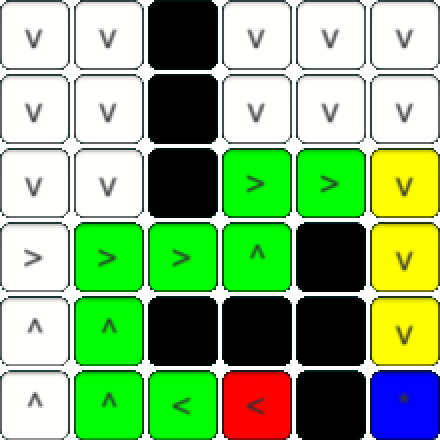
\includegraphics[width=1\textwidth]{images/OverlappingSubproblems/0.png}
\end{minipage}
\hfill
\begin{minipage}[t]{0.3\linewidth}
\centering
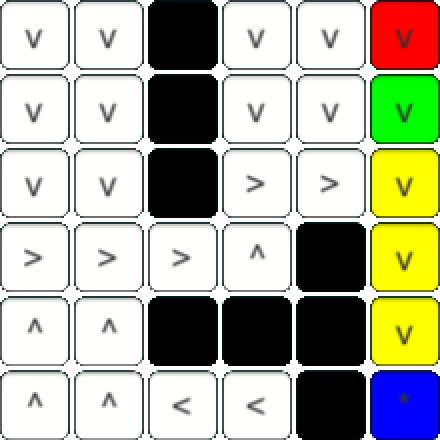
\includegraphics[width=1\textwidth]{images/OverlappingSubproblems/1.png}
\end{minipage}
\hfill
\begin{minipage}[t]{0.3\linewidth}
\centering
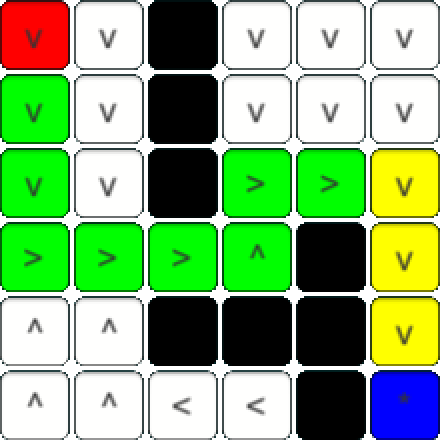
\includegraphics[width=1\textwidth]{images/OverlappingSubproblems/2.png}
\end{minipage}
\caption{An example of overlapping subproblems. In all three cases the yellow passage will be recalculated no matter from where you started (red). }
\end{figure}

\paragraph{Optimal substructure}
\quad \\
A problem has optimal substructure if the solution for the whole problem can be found by a combination of solutions for its subproblems. Normally, greedy algorithms are used to solve problems with this property because they lead to an optimal overall solution in this case. \cite{Cormen.2009}
\\
But also the principle of optimality is based in this idea.\\
To come back to the labyrinth, for any given position $p$ in the labyrinth a shortest path $s$ avoiding the walls and reaching a goal can be calculated. If $s$ is really the shortest path, it can be split into subpaths $s_1$ from $p$ to an point $x$ on the shortest path and $s_2$ from $x$ to the goal, such that $s_1, s_2$ are indeed the shortest paths between the three positions.\\
From that, a recursive way for finding shortest paths can easily be formulated, which is what is applied in Dynamic Programming.

\begin{figure}[h]
\centering
\begin{minipage}[t]{0.3\linewidth}
\centering
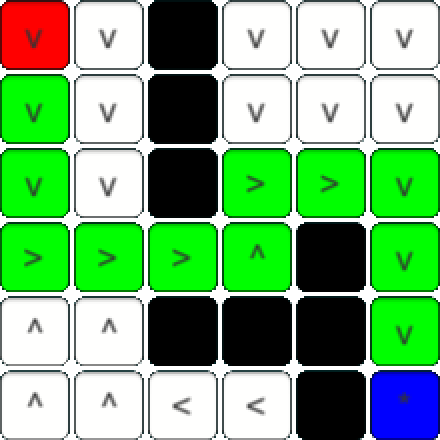
\includegraphics[width=1\textwidth]{images/OptimalSubstructure/start.png}
\caption{The overall shortest path $s$ (green) from start (red) to goal (blue).}
\end{minipage}
\hfill
\begin{minipage}[t]{0.3\linewidth}
\centering
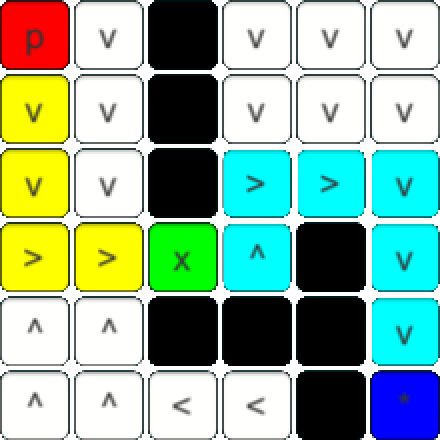
\includegraphics[width=1\textwidth]{images/OptimalSubstructure/first.png}
\caption{A first split of $s$ into $s_1$ (yellow) and $s_2$ (cyan).}
\end{minipage}
\hfill
\begin{minipage}[t]{0.3\linewidth}
\centering
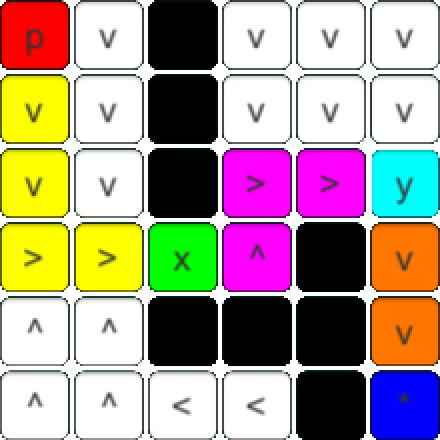
\includegraphics[width=1\textwidth]{images/OptimalSubstructure/second.png}
\caption{A second split of $s_2$ into $s_{2,1}$ (magenta) and $s_{2,2}$ (orange).}
\end{minipage}
\caption{An example of optimal substructure. The shortest path $s$ (green) can be split down into subproblems recursively until only the shortest path between two neighbored tiles has to be calculated. Based on these optimal solutions for the subproblems, the whole problem can be solved.}
\end{figure}

\subsubsection{How to apply Dynamic Programming in computer science}
\quad \\
\paragraph{Memoization}
\quad \\
An important concept when applying Dynamic Programming in computer science is memoization. As a result of the optimal substructure a problem can be broken down into simpler subproblems and for each of these subproblems, a solution can be calculated and the result can be stored in a table, so that a solution has to be found only once. When a subproblem reoccurs, the cached result can be returned to save computation time. \cite{Cormen.2009}
\\
On the other hand the storage consumption will expand due to the need for storing the results. But in times of rapidly increasing memory sizes and shrinking costs this draw off can often be considered as negligible. \cite{Cormen.2009}
\\
\paragraph{Bellman equation}
\quad \\
The Bellman equation, often also referred to as the Dynamic Programming equation, is a necessary condition for optimality.
It states a relationship between the value of a decision problem at a certain point in time depending on the outcome of the initial choices and the value of the remaining decisions that result from the previous choices. 
This breaks the problem down into subproblems that can be calculated seperately, as Bellman's principle of optimality suggests.\\
Before coming to the actual Bellman equation, some underlying concepts have to be defined.
At first, optimizing a problem is always under a certain objective: maximizing utility, minimizing path length, maximizing profits. The function describing these objectives is called the \textbf{objective function}.\\
Second, Dynamic Programming needs to keep track of the \textbf{state} of the system when evolving over time, because when breaking down a multi-period planning problem into simpler steps at different points in time, in every step the information about the current situation that is needed has to be available.\\
Furthermore, the next state is always affected by some factors in addition to the current \textbf{control}. That means, that choosing the control variables may be equivalent to choosing the action to reach the next state. This, in fact means making a decision.\\
In dynamic programming, an optimal plan can now be described by finding a rule that makes an interconnection between what the controls should be when given any possible value of the state. To now achieve the best possible value of the objective, the optimal decision rule has to be found.\\
Finally, by definition, the optimal decision rule is the one that achieves the best possible value of the objective. When written as a function of the state, the best possible value of the objective is called the \textbf{value function}.\\
Richard Bellman showed, that when calculating a relation between the value function of one step and the value function of the next step, a dynamic optimization problem can be solved in a recursive manner. The relationship connecting these two value functions is called the \textbf{Bellman equation} and uses an approach called \textbf{backwards induction}.\\
In this approach, the optimal policy of the last time period $t_N$ is specified at first as a function depending on the value of this state and the optimal value of the objective function.
Next, the previous step in time $t_{N-1}$ is calculated by optimizing the current ($t_{N-1}$) objective function and the optimal value for the future ($t_{N}$) objective function. This can be applied recursively until the initial state (t = 0) is reached and the first period decision rule is derived, as a function of the initial state and the value, by optimizing the sum of the objective function at the initial time step $t_{0}$ and the value of the second timestep $t_{1}$, which is dependent on all future decisions. Resulting from that, each periods decision is made by explicitly acknowledging that all future decisions will be optimally made.\\
So, when used on a dynamic decision problem the function describing the previously stated thoughts is
\begin{equation}
V(x_0) = \max_{a_0} \{F(x_0, a_0) + V(x_1)\}
\end{equation}
whereas $x_t$ is the state of the system at time $t$, beginning at $t = 0, x_0$ with
$a_0 \in \Gamma(x_0)$ being the action depending on the set of possible actions $\Gamma$ at $t_0$.
The transition from one state $x$ to another, is described by $T(x,a)$, when action $a$ is chosen at state $x$, and the payoff of taking $a$ in state $x$ is $F(x,a)$.
The Bellman equation can be simplified even more when dropping the time dependency resulting in a general functional equation
\begin{equation}
V(x) = \max_{a \in \Gamma(x)} \{F(x,a) + V(T(x,a))\}
\end{equation}
Solving this functional equation means now finding the unknown function V, which is the value function of the Problem. \cite{Bellman.2013}
\\

\section{Finding the value function and implementing the maze}
\subsection{Finding the value function}
Remember the initial task where you are given a grid map $M=\mathbb{N}^{nxm}$ containing static walls $M(i,j)=\infty$ representing the maze, and exit(s) of the labyrinth which the player wants to reach.\\
The goal of this paper is to point out ways to determine an optimal policy $P=\mathbb{N}^{nxm}\rightarrow A$ to exit the labyrinth by using Dynamic Programming. To achieve this, a way to calculate the value $v(i,j)$ of the current position is searched from what the actual best action can be derived.\\
To do so, we have to solve the Bellman equation for the task of finding all pair shortest paths in the maze.\\
This means, that for any arbitrary point in the maze a value function
\begin{equation}
v(i,j)\in \mathbb{N}
\end{equation}
representing the length of the shortest path of the position $(i, j)$ to the nearest goal in the maze has to be found.\\
Therefore let $c(i,j) \in \mathbb{R}$ be the cost it would take a prisoner in the maze to step on the field $(i,j)$.\\

So now let us at first begin with the trivial cases.\\
If a prisoner is already standing on a goal field, the cost to reach the goal would, obviously, be 
\begin{equation}
c(i,j) = 0, \quad \text{if } (i,j) \in \{X_\text{goal}\}
\end{equation}. 
Furthermore, also the value of a goal would be $0$, because the length of the shortest path from a position to itself is $0$.
In addition, if the prisoner isn't even in the maze, he will never be able to reach a goal, resulting in
\begin{equation}
v(i,j) = 
  \begin{cases}	
	\infty, \quad \text{if } i < 1 \text{ or } i > n \text{ or } j < 1 \text{ or } j > m \\
	0 \quad \quad \text{if } (i,j) \in \{X_\text{goal}\}
  \end{cases}
\end{equation}
At last if the position we're looking for is a wall, the cost is, by definition
\begin{equation}
c(i,j) = \infty, \quad if (i,j) \in \{Walls\}
\end{equation}
and the value of the tile is also $\infty$, because there will never be a payoff of stepping into a wall, because it isn't possible at all.
\\\\
Now to the non trivial cases.\\
Therefore let us have a look at a maze looking like

\begin{figure}[h]
\centering
\begin{minipage}[t]{0.3\linewidth}
\centering
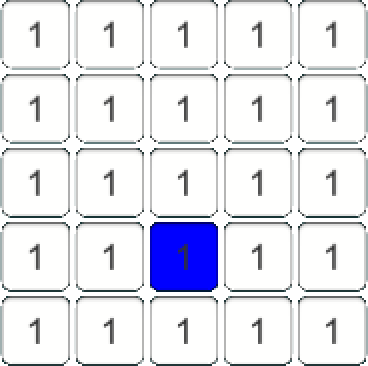
\includegraphics[width=1\textwidth]{images/ValueFunction/original.png}
\end{minipage}
\caption{All tiles are having a cost of
$1$.\\
$c(i,j) = 1, \quad \forall (i,j) \in n \times m$}
\end{figure}
Using the approach of backwards induction introduced by Richard Bellman we can start from the goal state in the grid and calculate the value at the step $N: v(3,4) = 0$.
Now having the result for $N$, we can induce backwards the results for the step $(N-1)$, whereas their results are
\begin{align}
v(2,4) = v(3,4) + c(3,4) = 0 + 1 = 1\\
v(4,4) = v(3,4) + c(3,4) = 0 + 1 = 1\\
v(2,3) = v(3,4) + c(3,4) = 0 + 1 = 1\\
v(2,5) = v(3,4) + c(3,4) = 0 + 1 = 1
\end{align}

When exemplary applying this procedure at the position $v(2,4)$, we can again give the equations for the positions lying around it
\begin{align}
v(1,4) = v(2,4) + c(2,4) = 1 + 1 = 2\\
v(3,4) = v(2,4) + c(2,4) = 1 + 1 = 2\\
v(2,3) = v(2,4) + c(2,4) = 1 + 1 = 2\\
v(2,5) = v(2,4) + c(2,4) = 1 + 1 = 2
\end{align}
Now we have calculated the values of the step $(N-2)$ depending on the decisions that will be made optimally in $(N-1) \text{ and } N$. The results are getting memoized in a second matrix $V^{n \times m}$ which is initialized with the value $\infty$ at all positions. So $V(3,4) = 0, V(2,4)=1 \dots$\\ 
One thing that has to be considered at this step is, that the value for the tile $v(3,4)$ is getting calculated again, which might cause troubles due to the fact that now the value of this position would be
\begin{equation}
v(3,4) = v(2,4) + c(2,4) = (v(3,4) + c(3,4)) + c(2,4) = 2
\end{equation}
which is in fact bigger than the initially calculated value of $0$. At this point we have to take into account if there is already a result of the value function memoized in the matrix $V$. If there is a result, and the value is less than the one currently calculated, the result can be discarded.\\

\begin{figure}[h]
\centering
\begin{minipage}[t]{0.3\linewidth}
\centering
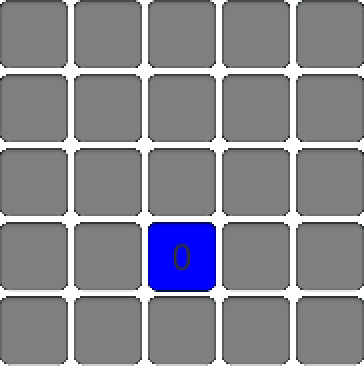
\includegraphics[width=1\textwidth]{images/ValueFunction/01.png}
\caption{Only the value of the goal position is known at step $N$.}
\end{minipage}
\hfill
\begin{minipage}[t]{0.3\linewidth}
\centering
\includegraphics[width=1\textwidth]{images/ValueFunction/02.png}
\caption{At step $(N-1)$ the values of the four adjacent positions are calculated.}
\end{minipage}
\hfill
\begin{minipage}[t]{0.3\linewidth}
\centering
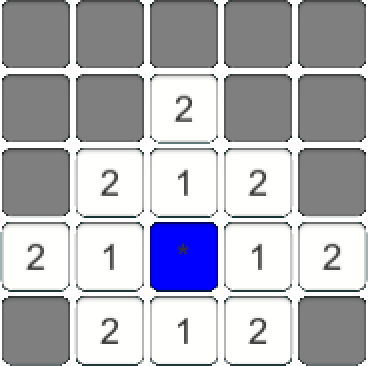
\includegraphics[width=1\textwidth]{images/ValueFunction/03.png}
\caption{At step $(N-2)$ the values of the positions adjacent to the previous positions are calculated.}
\end{minipage}
\caption{ }
\begin{minipage}[t]{0.3\linewidth}
\centering
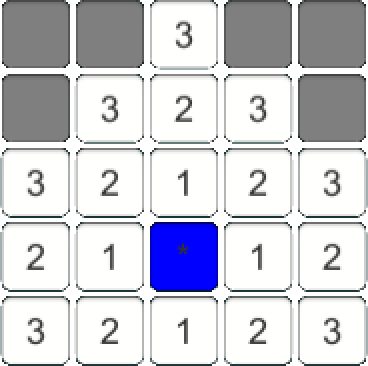
\includegraphics[width=1\textwidth]{images/ValueFunction/04.png}
\caption{Step $(N-3)$}
\end{minipage}
\hfill
\begin{minipage}[t]{0.3\linewidth}
\centering
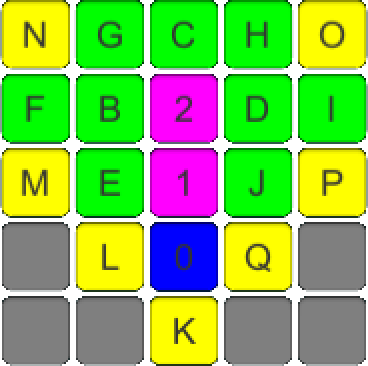
\includegraphics[width=1\textwidth]{images/ValueFunction/05.png}
\caption{Step $(N-4)$}
\end{minipage}
\hfill
\begin{minipage}[t]{0.3\linewidth}
\centering
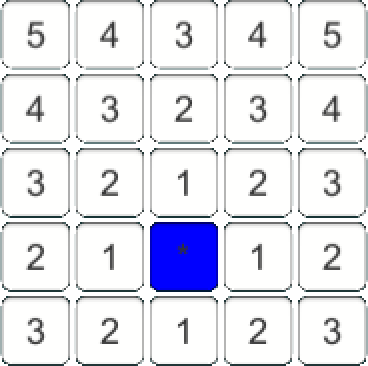
\includegraphics[width=1\textwidth]{images/ValueFunction/06.png}
\caption{At step $(N-5)$ the values of all the positions are calculated.}
\end{minipage}
\end{figure}

Following this procedure, a general relation between the steps can be stated:
\begin{align}
v(i-1,j) = v(i,j) + c(i,j) \quad \text{if } v(i-1,j) < V(i,j)\\
v(i+1,j) = v(i,j) + c(i,j) \quad \text{if } v(i+1,j) < V(i,j)\\
v(i,j-1) = v(i,j) + c(i,j) \quad \text{if } v(i,j-1) < V(i,j)\\
v(i,j+1) = v(i,j) + c(i,j) \quad \text{if } v(i,j+1) < V(i,j)
\end{align}

With these equations, the value of every position in the maze can be calculated.\\
When now solving the Bellman equation, a way to formulate the previous stated algorithm recursively has to be found.\\
In the backwards iterated method we started at the goal tile $(N)$ and derived the value of the positions adjacent to it $(N-1)$. On the opposite, we could have also started at the adjacent positions and look at the positions lying around them. For every position we want to find the position next to it, which holds the lowest sum of its value and its cost.\\
So for example when looking at the tile right of the goal state the four adjacent tiles would be observed. They would all but one have a value that is not yet calculated so we can't use these tiles to get a proper result. But the one tile that already has a value calculated is the goal tile lying left of this position. It's value would be $0$ as defined and it's cost would be $1$. So the value of the right adjacent tile would be $1$.\\
For the position on the top of the right tile, we could use the same method. Look at the four adjacent positions, find that some of the values aren't calculated yet and thereof can not be used but that there is one tile that is already calculated. So we could again add up the value and the cost to find the current value.\\
But what to do when coming to a tile that has more than one value next to it already calculated? Due to the fact that we want to find optimal policies and shortest paths, we want to minimize the value function. This can be achieved by deciding for the adjacent tile with the lowest value for itself. When now adding up it's value and it's cost, one can be sure to have calculated the lowest value for the tile.\\
Coming from this thought, it leads to the function solving the functional Bellman equation:

\begin{scriptsize}
\begin{equation}
v(i,j) =
  \begin{cases}
  \centering
    \infty & \text{if } (i,j) \in \{\text{Walls}\} \cup \{ \mathbb{R}^2 \setminus \{n \times m\}\}\\
    0 & \text{if } (i,j) \in \{\text{Goals}\}\\
    \min \{v(i,j+1) + c(i,j+1), \\v(i+1,j) + c(i+1,j), \\v(i,j-1) + c(i,j-1), \\v(i-1,j) + c(i-1,j)\} & \text{if in the maze and not a wall or a goal}
  \end{cases}
\end{equation}
\end{scriptsize}

\subsection{Finding optimal policies}
With the value of every tile calculated and stored in the matrix $V$, it is now trivial to find the optimal policy for any position.\\
Consider being at any position $x$ in the maze. All you can do is move into one of the four directions right, down, left and up. \\
Due to the fact that we are searching for the shortest path to the nearest goal, and the value of every tile is known, we can now make our decision where to step depending on the values of the tiles adjacent to the current position. By always choosing the tile with the lowest value, the best action $a \in A$ can be chosen accordingly.\\
Defined in a mathematical sense, the equation describing the value of every tile is the equation 
\begin{small}
\begin{align} 
\label{policy}
a(i,j)=
	\begin{cases}
		\text{up} \quad \quad \text{if } v(i,j-1) = \min_{(x,y)} \{v(x,y) + c(x,y)\} \\
		\text{right} \quad \text{if } v(i+1,j) = \min_{(x,y)} \{v(x,y) + c(x,y)\} \\
		\text{down} \quad \text{if } v(i,j+1) = \min_{(x,y)} \{v(x,y) + c(x,y)\} \\
		\text{left} \quad \quad \text{if } v(i-1,j) = \min_{(x,y)} \{v(x,y) + c(x,y)\} \\
	\end{cases} \\
	\text{With } (x,y) \in \{(i+1,j),(i-1,j),(i,j+1),(i,j-1)\}
\end{align}
\end{small}

\begin{figure}[h]
\centering
\begin{minipage}[t]{0.3\linewidth}
\centering
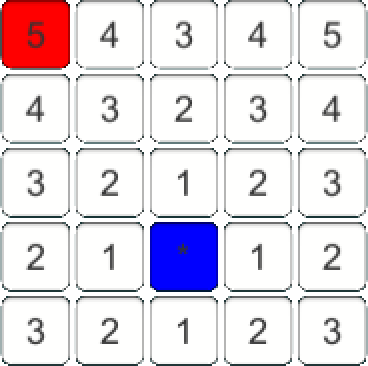
\includegraphics[width=1\textwidth]{images/FindingPolicy/01.png}
\caption{Starting from the red tile an optimal policy will be found.}
\end{minipage}
\hfill
\begin{minipage}[t]{0.3\linewidth}
\centering
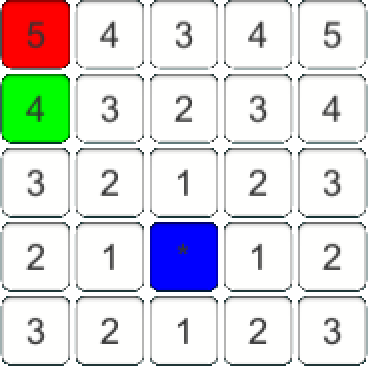
\includegraphics[width=1\textwidth]{images/FindingPolicy/02.png}
\caption{So looking at the adjacent tiles the green one is one of the tiles with the lowest value.}
\end{minipage}
\hfill
\begin{minipage}[t]{0.3\linewidth}
\centering
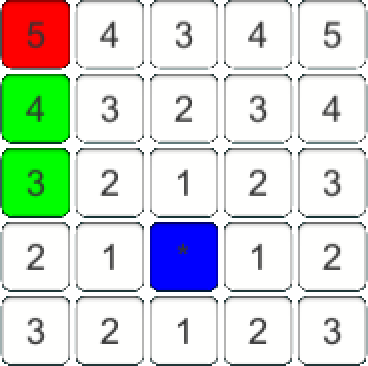
\includegraphics[width=1\textwidth]{images/FindingPolicy/03.png}
\caption{Following equation \ref{policy} a path is getting found.}
\end{minipage}
\caption{ }
\begin{minipage}[t]{0.3\linewidth}
\centering
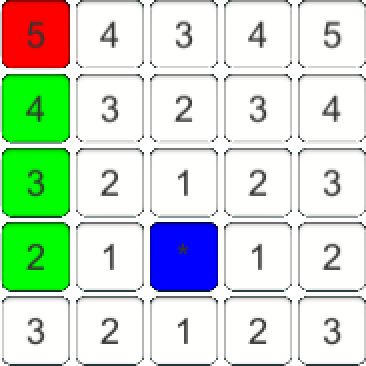
\includegraphics[width=1\textwidth]{images/FindingPolicy/04.png}
\caption{The path is reaching closer to the goal.}
\end{minipage}
\hfill
\begin{minipage}[t]{0.3\linewidth}
\centering
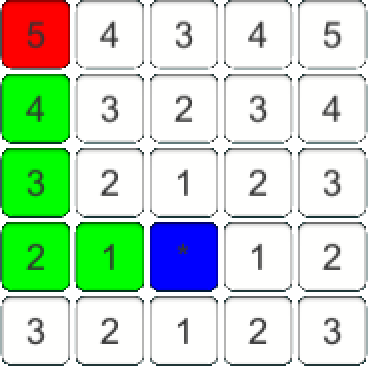
\includegraphics[width=1\textwidth]{images/FindingPolicy/05.png}
\caption{The path has reached the goal and the algorithm terminates returning one shortest path from red to blue.}
\end{minipage}
\hfill
\begin{minipage}[t]{0.3\linewidth}
\centering
\includegraphics[width=1\textwidth]{images/FindingPolicy/policy.png}
\caption{When \ref{policy} is applied to every tile, the best action at every position can be given.}
\end{minipage}
\end{figure}

%
%
%Now, if you moved onto one of these positions, you would have to pay the cost for each position and have to add it onto the value of this position. So making one of the steps, you would have to pay $1$. The resulting length of the shortest path now would be the value of the new position added to the cost it needed to step here.\\
%Now you could repeat this step and look at all the positions reachable from this position. As an example, let us look at the position $A$.\\
%One can now easily repeat these steps in an recursive way, summing up the cost until a goal is reached.\\
%So, if finally a goal state is reached, we would know that it's value is $0$, what would give us the possibility to calculate the values of the positions visited to reach it.\\
%
%To step on the goal, we would have to pay a cost of $1$ and the value of the goal is $0$. So summed up, for a tile that is in direct neighborhood of a goal state, it's value would be
%\begin{equation}
%v(i,j) = v(x,y) + 1, \quad (x,y) \in \{Goals\}
%\end{equation}
%This would propagate back until the initial position is reached.




%If you apply this approach to every position in the maze, you could calculate the value of every single position and from this grid of values, you could just always step on the position next to you which has the lowest cost which would result in a the optimal action for every tile in the maze.
%
%\begin{figure}[h]
%\centering
%\begin{minipage}[t]{0.3\linewidth}
%\centering
%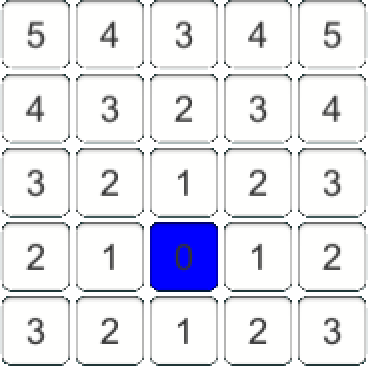
\includegraphics[width=1\textwidth]{images/ValueFunction/all.png}
%\caption{All values are found.}
%\end{minipage}
%\begin{minipage}{0.2\linewidth}
%\end{minipage}
%\begin{minipage}[t]{0.3\linewidth}
%\centering
%\includegraphics[width=1\textwidth]{images/ValueFunction/policy.png}
%\caption{Stepping onto the tile with the lowest value next to you, you can derive the best action.}
%\end{minipage}
%\end{figure}
%
%When coming to a mathematical representation of this problem, we saw that for every tile it's value was the value of the tile with the lowest cost next to it summed up with the cost it would take to step on this tile.\\
%From this the following function can be derived, which solves the Bellman equation.
%
%\begin{scriptsize}
%
%\begin{equation}
%v(i,j) =
%  \begin{cases}
%    \infty & \text{if } (i,j) \in \{\text{Walls}\} \cup \{ \mathbb{R}^2 \setminus \{n \times m\}\}\\
%    0 & \text{if } (i,j) \in \{\text{Goals}\}\\
%    \min \{v(i,j+1) + 1, \\v(i+1,j) + 1, \\v(i,j-1) + 1, \\v(i-1,j) + 1\} & \text{if in the maze and not a wall or a goal}
%  \end{cases}
%\end{equation}
%
%\end{scriptsize}
%
%The first to lines are the base cases to stop the recursion if a goal is found, the maze is left or a wall would be visited. If $n$ and $m$ are both finite numbers we can see that the recursion will always terminate because at some point in iterations the maze will be left in all directions which causes the calculation to stop.\\
%The third one is the recursive step searching for the minimum of the sum of the value of the four adjacent positions and their corresponding costs.\\
%If we now don't only allow $1$ as cost per tile, but also arbitrary positive values, the equation can be generalized to be used in any grid or graph with non negative costs.
%
%\begin{scriptsize}
%\begin{equation}
%v(i,j) =
%  \begin{cases}
%  \centering
%    \infty & \text{if } (i,j) \in \{\text{Walls}\} \cup \{ \mathbb{R}^2 \setminus \{n \times m\}\}\\
%    0 & \text{if } (i,j) \in \{\text{Goals}\}\\
%    \min \{v(i,j+1) + c(i,j+1), \\v(i+1,j) + c(i+1,j), \\v(i,j-1) + c(i,j-1), \\v(i-1,j) + c(i-1,j)\} & \text{if in the maze and not a wall or a goal}
%  \end{cases}
%\end{equation}
%\end{scriptsize}
%
%When the precomputation of the best action for every tile is finished, one can easily derive the optimal policy with ease.
%
%\begin{figure}[h]
%\centering
%\begin{minipage}[t]{0.3\linewidth}
%\centering
%\includegraphics[width=1\textwidth]{images/Policies/01.png}
%\caption{The optimal policy is $(\leftarrow,\leftarrow,\uparrow,\rightarrow,\rightarrow,$\\$\uparrow,\rightarrow,\rightarrow,\downarrow,\downarrow,\downarrow)$}
%\end{minipage}
%\hfill
%\begin{minipage}[t]{0.3\linewidth}
%\centering
%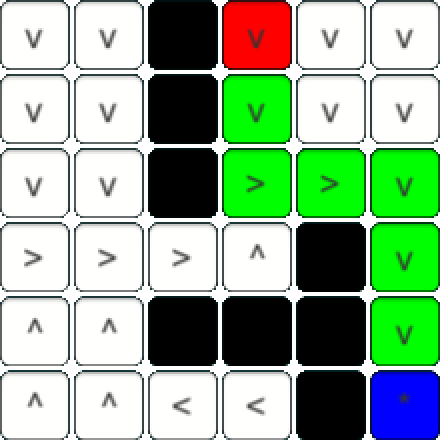
\includegraphics[width=1\textwidth]{images/Policies/02.png}
%\caption{The optimal policy is $(\downarrow,\downarrow,\rightarrow,\rightarrow,\downarrow,\downarrow,\downarrow)$}
%\end{minipage}
%\hfill
%\begin{minipage}[t]{0.3\linewidth}
%\centering
%\includegraphics[width=1\textwidth]{images/Policies/03.png}
%\caption{The optimal policy is $(\downarrow,\downarrow,\downarrow,\rightarrow,\rightarrow,\rightarrow,$\\$\uparrow,\rightarrow,\rightarrow,\downarrow,\downarrow,\downarrow)$}
%\end{minipage}
%\end{figure}
%
%\subsection{Pseudo code for solving this task}
%\begin{scriptsize}
%
%
%\lstset{
%  basicstyle=\ttfamily,
%  columns=fullflexible,
%  frame=single,
%  breaklines=true,
%  postbreak=\mbox{\textcolor{red}{$\hookrightarrow$}\space},
%  language=csh
%}
%\begin{lstlisting}
%
%public class Algorithm {
%
%private static int[,] grid;
%private static List<Vector2> goals;
%private static List<Vector2> openList = new List<Vector2>();
%
%public static void Recursive(int[,] grid, List<Vector2> goals){
%
%  Algorithm.grid = grid;
%  Algorithm.goals = goals;
%
%  value = new int[Width, Height];
%  policy = new char[Width, Height];
%
%  for (int i = 0; i < Width; i++)
%  {
%    for (int j = 0; j < Height; j++)
%      {
%        value[i, j] = MaxCost;
%      }
%  }
%
%  foreach (Vector2 goal in goals)
%  {
%    value[(int)goal.x, (int)goal.y] = 0;
%    policy[(int)goal.x, (int)goal.y] = '*';
%    ValueFunction(goal, new List<Vector2>() { goal });
%  }
%}
%
%
%
%private static void ValueFunction(Vector2 pos, List<Vector2> open/*, List<Vector2> closed*/){
%  open.Remove(pos);
%
%  for (int i = 0; i < deltas.Count; i++){
%    Vector2 prev = pos - deltas[i];
%    if (prev.x >= 0 && prev.x < Width && prev.y >= 0 && prev.y < Height)
%    {
%      if (grid[(int)prev.x, (int)prev.y] == MaxCost)
%      {
%        value[(int)prev.x, (int)prev.y] = MaxCost;
%      }
%      else if (goals.Contains(prev))
%      {
%        value[(int)prev.x, (int)prev.y] = 0;
%      }
%      else if (value[(int)prev.x, (int)prev.y] > value[(int)pos.x, (int)pos.y] + grid[(int)pos.x, (int)pos.y])
%      {
%        if (!open.Contains(prev))
%          open.Add(prev);
%
%        if (goals.Contains(prev))
%        {
%          value[(int)prev.x, (int)prev.y] = 0;
%          policy[(int)prev.x, (int)prev.y] = '*';
%        }
%        else
%        {
%          value[(int)prev.x, (int)prev.y] = value[(int)pos.x, (int)pos.y] + grid[(int)pos.x, (int)pos.y];
%          policy[(int)prev.x, (int)prev.y] = deltaNames[i];
%        }
%      }
%    }
%  }
%
%  //Sort list
%  if (open.Count > 0)
%  {
%    int index = -1;
%    int lowest = int.MaxValue;
%    for (int i = 0; i < open.Count; i++)
%    {
%      if (value[(int)open[i].x, (int)open[i].y] + grid[(int)pos.x, (int)pos.y] < lowest)
%      {
%        lowest = value[(int)open[i].x, (int)open[i].y];
%        index = i;
%      }
%    }
%    ValueFunction(open[index], open/*, closed*/);
%  }
%}
%
%}
%\end{lstlisting}
%\end{scriptsize}
\section{Related Work}
\subsection{Autonomous vehicles}
As cars being just one special type of robots, finding the navigation paths has been a field with many research dedicated to. They have to go straight, take turns, switch lanes and always avoid collisions with pedestrians or other cars.\\
Classic algorithms like Dijkstras algorithm or based on it A* are a very prominent example of algorithms solving these tasks. But their disadvantage is often the fact that they only solve the shortest path problem for the current location to the nearest goal.\\
The huge advantage Dynamic Programming brings to the field of autonomous driving is that with the calculation of optimal policies a best action for every position on the map can be calculated previously, so that even if there is an unexpected obstacle blocking a lane shift or a turn and resulting in being in a position not in the optimal shortest path, a alternative solution is already calculated.\\
But also for smaller autonomous robots like vacuum robots dynamic programming is a nice way to navigate. A map of the room has to be given or found by the little helper based on which it can then define solid obstacles like tables or cupboards, whereas goals can be defined as dirt hotspots or the loading station for the robot.\\


\subsection{Extending the 2-dimensional algorithms onto N-dimensional problems}
But how can the Dynamic Programming approach be used for robot motion planning with more than 2 dimensions? Imagine a two-armed robot having six degrees of freedom for every arm resulting in a 12-dimensional motion planning problem.\\
For every possible configuration of the arms a node in a graph $G$ can be defined holding the specific attributes of that configuration. For every transition between two configurations an edge between these two can be drawn describing uniquely the transformation between the two states.\\
With this approach every N-dimensional problem can be projected down onto a two-dimensional plane where the algorithms can easily be applied.\\
Based on this method many robot motion planning algorithms have been introduced.

\subsection{Algorithmic Design of Feasible Trajectories}
Written by Steven M. LaValle, this paper summarizes the recent development of algorithms that construct feasible trajectories made at the University of Illinois. They use et al dynamic programming approaches that produce approximately-optimal solutions for low-dimensional problems. \\
The difficulties they had to come over are on the one side differential constraints, which means that in a systems the number of actuators is strictly less than the dimension of the configuration space. For example imagine a spacecraft floating in $\mathbb{R}^3$ that has three thrusters. These are called the actuators of the spacecraft system. Opposite, the spacecraft has six degrees of freedom (X-Pos., Y-Pos., Z-Pos., Yaw, Pitch, Roll) which makes it an underactuated system having differential constraints.\\
On the other hand they had to deal with global constraints arising from robot collisions.\\
%\subsubsection{problem formulation}
%\begin{enumerate}
%\item State Space: $X \subset \mathbb{R}^n$
%\item Boundary Values: $x_\text{init} \in X, X_\text{goal} \subset X$
%\item Contraint Satisfaction: A function, $D : X \rightarrow \{\text{true, false}\}$, that determines wheater global constraints are satisfied from state $x$.
%\item Inputs: $U(x) \subset \mathbb{R}^m, \forall x \in X$, which specifies the set of controls.
%\item State Transition Equation: $\dot{x} = f(x, u)$
%\end{enumerate}
\subsubsection{Dynamic Programming}
\quad \\
Using Bellman's principle of optimality, let $k$ refer to a \textit{stage} or \textit{time step}, and let $x_k$ and $u_k$ refer to the state and input at stage $k$. For their purpose $K+1$ represented the final stage.\\
The cost function used to describe this problem is of the form
\begin{equation}
L(x_1,\cdots,x_{K+1}, u_1,\cdots,u_K) = \sum_{k=1}^K l(x_k,u_k) + l_{K+1}(x_{K+1})
\end{equation}
whereas $l_{K+1}(x_{K+1})=0$ if $x_{K+1} \in X_\text{goal}$, and $l_{K+1}(x_{K+1})=\infty$ else.\\
They used classical Cost-to-go Iterations that can solve this problem numerically, whereas the cost-to-go function they used is 
\begin{equation}
L_k^*(x_k) = \min_{u_k,\cdots,u_K} \left\{ \sum_{i=k}^K l(x_i,u_i)+l_{K+1}(x_{K+1})\right\}.
\end{equation}
This now induces the calculation of the cost-to-go functions iteratively from stage $K+1$ to $1$. In each iteration, $L_k^*$ is computed using the result of $L_{K+1}^*$ by using the following dynamic programming equation, which involves a local optimization over the inputs:
\begin{equation}
L_k^*(x_k) = \min_{u_k} \left\{l(x_k,u_k) + L_{K+1}^*(x_{K+1})\right\}.
\end{equation}
For further reading see \cite{LaValle.}

\subsection{Rapidly exploring Random Trees (RRT)}
\subsubsection{What is a RRT}
\quad \\
Another very interesting field of research are Rapidly-exploring Random Trees, which were first introduced by LaValle in October 1998 \cite{LaValle.October1998}.\\
The main idea behind RRTs is a randomized data structure that is designed for a broad class of path planning problems that are viewed as search in a metric space X for a continuous path from an initial state $x_{\text{init}}$ to a goal region $X_\text{goal} \subset X$\\
In addition, a fixed obstacle region $X_\text{obs} \subset X$ must be avoided, but there is no explicit representation of it available, thus one can only check if a specific state lies in $X_\text{obs}$.\\
The nice thing about RRTs is, that $X_\text{obs}$ not only represents solid obstacles like walls, trees or blocks, but can represent any type of constraints. These include velocity bounds of a self-driving car, configurations at which a robot is in collision with an obstacle in the world and any other constraints occurring in motion planning problems.\\
When constructing the RRT, the vertices represent the states of the system in $X_\text{free}$, and each edge will correspond to a path that lies in completely in $X_\text{free}$. \cite{LaValle.October1998}\\

\subsubsection{How does a RRT look like and how to construct}
\begin{enumerate}
\item Pick a random sample in the search space.
\item Find the nearest neighbor of that sample.
\item Select an action from the neighbor that heads towards the random sample.
\item Create a new sample based on the outcome of the action applied to the neighbor.
\item Add the new sample to the tree, and connect it to the neighbor.
\end{enumerate}

\begin{figure}[h]
\centering
\begin{minipage}[t]{0.3\linewidth}
\centering
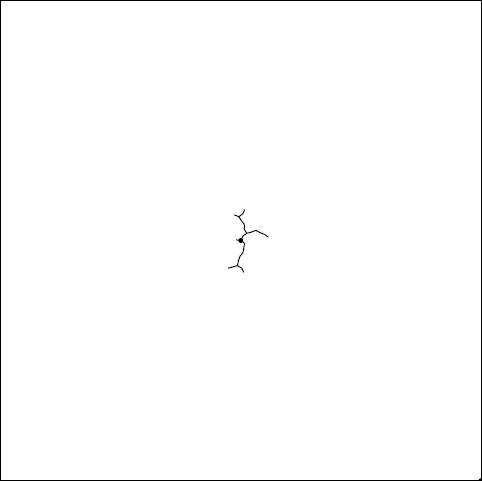
\includegraphics[width=1\textwidth]{images/RRT/01.png}
\caption{At the beginning the search space is completely unexplored. The tree begins spanning into it.}
\end{minipage}
\hfill
\begin{minipage}[t]{0.3\linewidth}
\centering
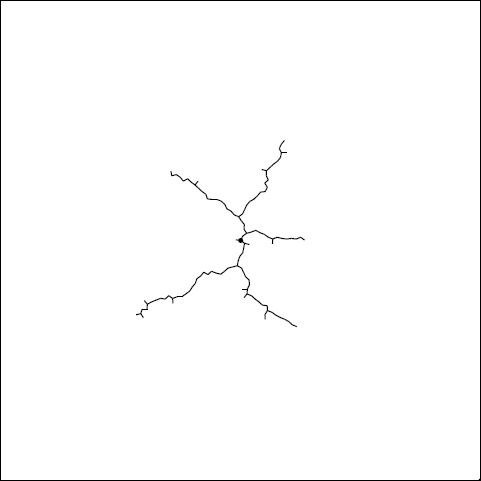
\includegraphics[width=1\textwidth]{images/RRT/02.png}
\caption{The tree reaches further into the unexplored space.}
\end{minipage}
\hfill
\begin{minipage}[t]{0.3\linewidth}
\centering
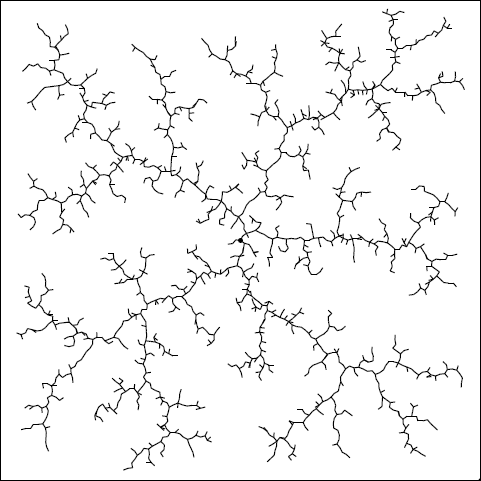
\includegraphics[width=1\textwidth]{images/RRT/03.png}
\caption{The tree is reaching to the limits of the plane and is getting denser. At the limit it will have covered the whole $X_\text{free}$}
\end{minipage}
\\
\begin{minipage}[t]{0.3\linewidth}
\centering
\includegraphics[width=1\textwidth]{images/RRT/01_v.png}
\caption{Looking at the voronoi bias of the vertices, there are huge unexplored parts.}
\end{minipage}
\hfill
\begin{minipage}[t]{0.3\linewidth}
\centering
\includegraphics[width=1\textwidth]{images/RRT/02_v.png}
\caption{The tree is always taking a sample out of the biggest unexplored part. This smallers the part.}
\end{minipage}
\hfill
\begin{minipage}[t]{0.3\linewidth}
\centering
\includegraphics[width=1\textwidth]{images/RRT/03_v.png}
\caption{When proceeding, the voronoi bias are simultaneously getting smaller with every iteration. Their area tends to be 0 at the limit.}
\end{minipage}
\end{figure}
\cite{LaValle.October1998}, \cite{OktayArslan.December2015}
\subsubsection{RRTs and dynamic programming}
\quad \\
In the dissertation of Oktay Arslan at the Georgia Institute of Technology in December 2015, he gives a extension of the solely sampling based approach of the original RRT.\\
He introduces an algorithm called $\text{RRT}^\#$ which utilizes the main ideas from RRT, but expanded it with a relaxation step which uses Dynamic Programming.\\
Relaxation is a term used iterative methods for solving systems of equations, in this case of optimization problems in numerical mathematics.\\
They can be written down in the form of
\begin{equation}
x(k+1) = f(x(k)), \quad k = 0,1,\cdots
\end{equation}
where $x(k) \in \mathbb{R}^n$ is an n-dimensional vector, and $f : \mathbb{R}^n \mapsto \mathbb{R}^n$ is a vector-valued function.\\
The Bellman function is of this form, what spans the bow between Dynamic Programming and $\text{RRT}^\#$.\\
For understanding the algorithm, some concepts have to be defined:
\begin{itemize}
%\item Successor vertices: Given a vertex $v \in V$ in a directed Graph $G = (V,E)$, the function $\text{succ} : (G,v) \mapsto V' \subseteq V$ returns the vertices in $V$ that can be reached from vertex v.
%\begin{center}
%$\text{succ}(G,v) := \{u \in V: (v,u) \in E\}$
%\end{center}
\item Predecessor vertices: Given a vertex $v \in V$ in a directed Graph $G = (V,E)$, the function $\text{pred} : (G,v) \mapsto V' \subseteq V$ returns the vertices in $V$ from which vertex v can be reached.
\begin{center}
$\text{pred}(G,v) := \{u \in V: (v,u) \in E\}$
\end{center}
\end{itemize}
Following thereof, they rewrote the bellman equation for their purpose in terms of the cost-to-come value as follows:
\begin{small}
\begin{equation}
g^*(v_i) = 
\begin{cases}
0 & v_i = x_\text{init}\\
\min_{v_j \in pred(G,v_i)} (g^*(v_j) + c(v_j,v_i)) & v_i \in V \setminus \{x_\text{init}\}
\end{cases}
\end{equation}
\end{small}
Based on their formulation of the Bellman equation, they split the Algorithm into two parts:\\
\paragraph{Exploration}
This samples randomly a point in $X_\text{free}$ and then extends the underlying graph towards the sampled point by including it as a new vertex in the current graph by connecting the missing edges. \cite{OktayArslan.December2015}\\
\paragraph{Exploitation}
In this step the explored graph is getting refined by finding promising vertices. The values of these vertices are updated and unnecessary ties are broken so that the algorithm only expands vertices that are very likely to lie on the shortest path.

The following images show the two algorithms.

\begin{figure}[h]
\centering
\begin{minipage}[t]{0.3\linewidth}
\centering
\includegraphics[width=1\textwidth]{images/RRT/ARSLAN/01.png}
\caption{The tree after 250 iterations}
\end{minipage}
\hfill
\begin{minipage}[t]{0.3\linewidth}
\centering
\includegraphics[width=1\textwidth]{images/RRT/ARSLAN/02.png}
\caption{The tree after 2500 iterations}
\end{minipage}
\hfill
\begin{minipage}[t]{0.3\linewidth}
\centering
\includegraphics[width=1\textwidth]{images/RRT/ARSLAN/03.png}
\caption{The tree after 25000 iterations}
\end{minipage}
\caption{The evolution of the tree computed by RRT, the original algorithm. The tree is spanning equally in all directions resulting in a uniform density.}
\end{figure}

\begin{figure}[h]
\centering
\begin{minipage}[t]{0.3\linewidth}
\centering
\includegraphics[width=1\textwidth]{images/RRT/ARSLAN/01_v.png}
\caption{The tree after 250 iterations}
\end{minipage}
\hfill
\begin{minipage}[t]{0.3\linewidth}
\centering
\includegraphics[width=1\textwidth]{images/RRT/ARSLAN/02_v.png}
\caption{The tree after 2500 iterations}
\end{minipage}
\hfill
\begin{minipage}[t]{0.3\linewidth}
\centering
\includegraphics[width=1\textwidth]{images/RRT/ARSLAN/03_v.png}
\caption{The tree after 25000 iterations}
\end{minipage}
\caption{The evolution of the tree computed by $\text{RRT}^\#$. The tree is spanning mostly into the direction of the promising vertices. The density around the shortest path is much higher than in the regions not associated with it.}
\end{figure}

In the uniform distribution of the original RRT the computation time is mostly wasted for vertices that have no chance of being part of the shortest path. Due to the fact that in $\text{RRT}^\#$ only the promising vertices are expanded and not promising ones are left, the density around the shortest path is really high. Thereof $\text{RRT}^\#$ safes the time and effort wasted by the original RRT and uses it only on the promising vertices resulting in a huge improvement in runtime and memory usage.
The interested reader can have a look at \cite{OktayArslan.December2015} for further information and mathematical proofs.

%\subsection{Bellman Ford, Gauss Seidel and Jakobi}

\section{Conclusion}
As we have seen in this paper, Dynamic Programming is a very straight forward approach for solving multistage decision problems. By breaking down difficult problems into sets of overlapping subproblems with optimal substructure an overall optimal solution can be found by only solving the small subproblems. In robot motion, dynamic programming can be applied in a wide field of tasks and can be a really useful approach that takes the place of the classic algorithms.
Many algorithms are already getting improved or replaced by Dynamic Programming algorithms and the set of fields where it can be applied is nearly unlimited.



%-----------------------------------------------------------------
%Image Template
%-----------------------------------------------------------------
%\quad \\
%\begin{figure}[h]
%\centering
%\begin{minipage}[t]{0.3\linewidth}
%\centering
%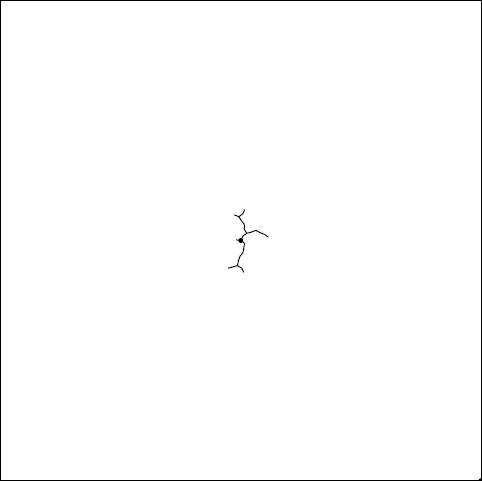
\includegraphics[width=1\textwidth]{images/RRT/01.png}
%\caption{}
%\end{minipage}
%\hfill
%\begin{minipage}[t]{0.3\linewidth}
%\centering
%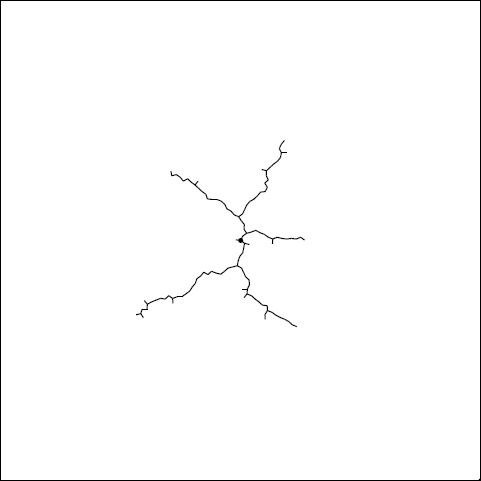
\includegraphics[width=1\textwidth]{images/RRT/02.png}
%\caption{}
%\end{minipage}
%\hfill
%\begin{minipage}[t]{0.3\linewidth}
%\centering
%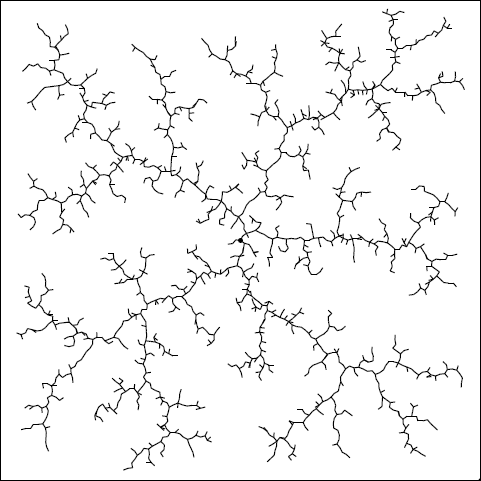
\includegraphics[width=1\textwidth]{images/RRT/03.png}
%\caption{}
%\end{minipage}
%\caption{}
%\end{figure}






% An example of a floating figure using the graphicx package.
% Note that \label must occur AFTER (or within) \caption.
% For figures, \caption should occur after the \includegraphics.
% Note that IEEEtran v1.7 and later has special internal code that
% is designed to preserve the operation of \label within \caption
% even when the captionsoff option is in effect. However, because
% of issues like this, it may be the safest practice to put all your
% \label just after \caption rather than within \caption{}.
%
% Reminder: the "draftcls" or "draftclsnofoot", not "draft", class
% option should be used if it is desired that the figures are to be
% displayed while in draft mode.
%
%\begin{figure}[!t]
%\centering
%\includegraphics[width=2.5in]{myfigure}
% where an .eps filename suffix will be assumed under latex, 
% and a .pdf suffix will be assumed for pdflatex; or what has been declared
% via \DeclareGraphicsExtensions.
%\caption{Simulation Results.}
%\label{fig_sim}
%\end{figure}

% Note that IEEE typically puts floats only at the top, even when this
% results in a large percentage of a column being occupied by floats.


% An example of a double column floating figure using two subfigures.
% (The subfig.sty package must be loaded for this to work.)
% The subfigure \label commands are set within each subfloat command,
% and the \label for the overall figure must come after \caption.
% \hfil is used as a separator to get equal spacing.
% Watch out that the combined width of all the subfigures on a 
% line do not exceed the text width or a line break will occur.
%
%\begin{figure*}[!t]
%\centering
%\subfloat[Case I]{\includegraphics[width=2.5in]{box}%
%\label{fig_first_case}}
%\hfil
%\subfloat[Case II]{\includegraphics[width=2.5in]{box}%
%\label{fig_second_case}}
%\caption{Simulation results.}
%\label{fig_sim}
%\end{figure*}
%
% Note that often IEEE papers with subfigures do not employ subfigure
% captions (using the optional argument to \subfloat[]), but instead will
% reference/describe all of them (a), (b), etc., within the main caption.


% An example of a floating table. Note that, for IEEE style tables, the 
% \caption command should come BEFORE the table. Table text will default to
% \footnotesize as IEEE normally uses this smaller font for tables.
% The \label must come after \caption as always.
%
%\begin{table}[!t]
%% increase table row spacing, adjust to taste
%\renewcommand{\arraystretch}{1.3}
% if using array.sty, it might be a good idea to tweak the value of
% \extrarowheight as needed to properly center the text within the cells
%\caption{An Example of a Table}
%\label{table_example}
%\centering
%% Some packages, such as MDW tools, offer better commands for making tables
%% than the plain LaTeX2e tabular which is used here.
%\begin{tabular}{|c||c|}
%\hline
%One & Two\\
%\hline
%Three & Four\\
%\hline
%\end{tabular}
%\end{table}


% Note that IEEE does not put floats in the very first column - or typically
% anywhere on the first page for that matter. Also, in-text middle ("here")
% positioning is not used. Most IEEE journals/conferences use top floats
% exclusively. Note that, LaTeX2e, unlike IEEE journals/conferences, places
% footnotes above bottom floats. This can be corrected via the \fnbelowfloat
% command of the stfloats package.






% conference papers do not normally have an appendix


% use section* for acknowledgement
% \section*{Acknowledgment}
% The authors would like to thank...





% trigger a \newpage just before the given reference
% number - used to balance the columns on the last page
% adjust value as needed - may need to be readjusted if
% the document is modified later
%\IEEEtriggeratref{8}
% The "triggered" command can be changed if desired:
%\IEEEtriggercmd{\enlargethispage{-5in}}



% references section
\newpage
% can use a bibliography generated by BibTeX as a .bbl file
% BibTeX documentation can be easily obtained at:
% http://www.ctan.org/tex-archive/biblio/bibtex/contrib/doc/
% The IEEEtran BibTeX style support page is at:
% http://www.michaelshell.org/tex/ieeetran/bibtex/
\bibliographystyle{IEEEtran}
% argument is your BibTeX string definitions and bibliography database(s)
%\nocite{*}
%\bibliography{Docs/Literatur}
%
% <OR> manually copy in the resultant .bbl file
% set second argument of \begin to the number of references
% (used to reserve space for the reference number labels box)
% Generated by IEEEtran.bst, version: 1.14 (2015/08/26)


% Generated by IEEEtran.bst, version: 1.14 (2015/08/26)
%\begin{thebibliography}{10}
%\providecommand{\url}[1]{#1}
%\csname url@samestyle\endcsname
%\providecommand{\newblock}{\relax}
%\providecommand{\bibinfo}[2]{#2}
%\providecommand{\BIBentrySTDinterwordspacing}{\spaceskip=0pt\relax}
%\providecommand{\BIBentryALTinterwordstretchfactor}{4}
%\providecommand{\BIBentryALTinterwordspacing}{\spaceskip=\fontdimen2\font plus
%\BIBentryALTinterwordstretchfactor\fontdimen3\font minus
%  \fontdimen4\font\relax}
%\providecommand{\BIBforeignlanguage}[2]{{%
%\expandafter\ifx\csname l@#1\endcsname\relax
%\typeout{** WARNING: IEEEtran.bst: No hyphenation pattern has been}%
%\typeout{** loaded for the language `#1'. Using the pattern for}%
%\typeout{** the default language instead.}%
%\else
%\language=\csname l@#1\endcsname
%\fi
%#2}}
%\providecommand{\BIBdecl}{\relax}
%\BIBdecl
%
%\bibitem{OktayArslan.December2015}
%\BIBentryALTinterwordspacing
%O.~Arslan, ``Machine learning and dynamic programming algorithms for motion
%  planning and control,'' 2015-12-01. [Online]. Available:
%  \url{http://hdl.handle.net/1853/54317}
%\BIBentrySTDinterwordspacing
%
%\bibitem{Bellman.30.07.1954}
%\BIBentryALTinterwordspacing
%R.~Bellman, ``The theory of dynamic programming,'' {The RAND Corporation},
%  1954. [Online]. Available:
%  \url{https://www.rand.org/content/dam/rand/pubs/papers/2008/P550.pdf}
%\BIBentrySTDinterwordspacing
%
%\bibitem{LaValle.}
%\BIBentryALTinterwordspacing
%S.~LaValle, ``From dynamic programming to rrts: Algorithmic design of feasible
%  trajectories,'' {University of Illinois}. [Online]. Available:
%  \url{http://msl.cs.illinois.edu/~lavalle/papers/Lav02.pdf}
%\BIBentrySTDinterwordspacing
%
%\bibitem{LaValle.October1998}
%\BIBentryALTinterwordspacing
%------, ``Rapidly-exploring random trees: A new tool for path planning,'' {Iowa
%  State University}, October 1998. [Online]. Available:
%  \url{http://msl.cs.illinois.edu/~lavalle/papers/Lav98c.pdf}
%\BIBentrySTDinterwordspacing
%
%\bibitem{Bellman.1953}
%R.~Bellman, ``On the theory of dynamic programming,'' {The RAND Corporation},
%  1952.
%
%\bibitem{Bellman.1958}
%\BIBentryALTinterwordspacing
%------, ``On a routing problem,'' vol.~16, pp. 87--90, 1958. [Online].
%  Available: \url{http://www.jstor.org/stable/43634538}
%\BIBentrySTDinterwordspacing
%
%\bibitem{Bellman.2013}
%\BIBentryALTinterwordspacing
%------, \emph{\BIBforeignlanguage{eng}{Dynamic Programming}}, ser. Dover Books
%  on Computer Science.\hskip 1em plus 0.5em minus 0.4em\relax {Dover
%  Publications}, 2013. [Online]. Available:
%  \url{http://gbv.eblib.com/patron/FullRecord.aspx?p=1897424}
%\BIBentrySTDinterwordspacing
%
%\bibitem{Bradley.1992}
%S.~P. Bradley, A.~C. Hax, and T.~L. Magnanti,
%  \emph{\BIBforeignlanguage{eng}{Applied mathematical programming}}, [19.
%  dr.]~ed.\hskip 1em plus 0.5em minus 0.4em\relax Addison-Wesley, 1992, hax,
%  Arnoldo C. (VerfasserIn) Magnanti, Thomas L. (VerfasserIn).
%
%\bibitem{Cooke.1966}
%\BIBentryALTinterwordspacing
%K.~L. Cooke and E.~Halsey, ``The shortest route through a network with
%  time-dependent internodal transit times,'' vol.~14, pp. 493--498, 1966.
%  [Online]. Available:
%  \url{http://www.sciencedirect.com/science/article/pii/0022247X66900096}
%\BIBentrySTDinterwordspacing
%
%\bibitem{Cormen.2007}
%T.~H. Cormen, \emph{\BIBforeignlanguage{eng}{Introduction to algorithms}},
%  2nd~ed.\hskip 1em plus 0.5em minus 0.4em\relax {MIT Press}, 2007.
%
%\bibitem{Derigs.1995}
%``Operations research proceedings 1994: Selected papers of the international
%  conference on operations research, berlin, august 30 -- september 2, 1994,''
%  1995.
%
%\bibitem{Dreyfus.2002}
%\BIBentryALTinterwordspacing
%S.~Dreyfus, ``Richard bellman on the birth of dynamic programming,'' vol.~50,
%  pp. 48--51, 2002. [Online]. Available:
%  \url{https://doi.org/10.1287/opre.50.1.48.17791}
%\BIBentrySTDinterwordspacing
%
%\bibitem{LaValle.2006Referencesfromthebook}
%S.~M. LaValle, \emph{Planning Algorithms}.\hskip 1em plus 0.5em minus
%  0.4em\relax {Cambridge University Press}, 2006 {\%} References from the book,
%  available at http://planning.cs.uiuc.edu/.
%
%\bibitem{Pra.1995}
%\BIBentryALTinterwordspacing
%P.~D. Pra, C.~Rudari, and W.~J. Runggaldier, ``On dynamic programming for
%  multistage decision problems under uncertainty,'' in \emph{Operations
%  Research Proceedings 1994: Selected Papers of the International Conference on
%  Operations Research, Berlin, August 30 -- September 2, 1994}, U.~Derigs,
%  A.~Bachem, and A.~Drexl, Eds.\hskip 1em plus 0.5em minus 0.4em\relax
%  {Springer Berlin Heidelberg}, 1995, pp. 70--75. [Online]. Available:
%%  \url{https://doi.org/10.1007/978-3-642-79459-9_14}
%\BIBentrySTDinterwordspacing
%
%\end{thebibliography}


% Generated by IEEEtran.bst, version: 1.14 (2015/08/26)
\begin{thebibliography}{10}
\providecommand{\url}[1]{#1}
\csname url@samestyle\endcsname
\providecommand{\newblock}{\relax}
\providecommand{\bibinfo}[2]{#2}
\providecommand{\BIBentrySTDinterwordspacing}{\spaceskip=0pt\relax}
\providecommand{\BIBentryALTinterwordstretchfactor}{4}
\providecommand{\BIBentryALTinterwordspacing}{\spaceskip=\fontdimen2\font plus
\BIBentryALTinterwordstretchfactor\fontdimen3\font minus
  \fontdimen4\font\relax}
\providecommand{\BIBforeignlanguage}[2]{{%
\expandafter\ifx\csname l@#1\endcsname\relax
\typeout{** WARNING: IEEEtran.bst: No hyphenation pattern has been}%
\typeout{** loaded for the language `#1'. Using the pattern for}%
\typeout{** the default language instead.}%
\else
\language=\csname l@#1\endcsname
\fi
#2}}
\providecommand{\BIBdecl}{\relax}
\BIBdecl

\bibitem{OktayArslan.December2015}
\BIBentryALTinterwordspacing
O.~Arslan, ``Machine learning and dynamic programming algorithms for motion
  planning and control,'' 2015-12-01. [Online]. Available:
  \url{http://hdl.handle.net/1853/54317}
\BIBentrySTDinterwordspacing

\bibitem{Dreyfus.2002}
\BIBentryALTinterwordspacing
S.~Dreyfus, ``Richard bellman on the birth of dynamic programming,'' vol.~50,
  pp. 48--51, 2002. [Online]. Available:
  \url{https://doi.org/10.1287/opre.50.1.48.17791}
\BIBentrySTDinterwordspacing

\bibitem{Bellman.30.07.1954}
\BIBentryALTinterwordspacing
R.~Bellman, ``The theory of dynamic programming,'' {The RAND Corporation},
  1954. [Online]. Available:
  \url{https://www.rand.org/content/dam/rand/pubs/papers/2008/P550.pdf}
\BIBentrySTDinterwordspacing

\bibitem{Bellman.2013}
\BIBentryALTinterwordspacing
------, \emph{\BIBforeignlanguage{eng}{Dynamic Programming}}, ser. Dover Books
  on Computer Science.\hskip 1em plus 0.5em minus 0.4em\relax {Dover
  Publications}, 2013. [Online]. Available:
  \url{http://gbv.eblib.com/patron/FullRecord.aspx?p=1897424}
\BIBentrySTDinterwordspacing

\bibitem{LaValle.}
\BIBentryALTinterwordspacing
S.~LaValle, ``From dynamic programming to rrts: Algorithmic design of feasible
  trajectories,'' {University of Illinois}. [Online]. Available:
  \url{http://msl.cs.illinois.edu/~lavalle/papers/Lav02.pdf}
\BIBentrySTDinterwordspacing

\bibitem{LaValle.October1998}
\BIBentryALTinterwordspacing
------, ``Rapidly-exploring random trees: A new tool for path planning,'' {Iowa
  State University}, October 1998. [Online]. Available:
  \url{http://msl.cs.illinois.edu/~lavalle/papers/Lav98c.pdf}
\BIBentrySTDinterwordspacing

\bibitem{Bellman.1953}
R.~Bellman, ``On the theory of dynamic programming,'' {The RAND Corporation},
  1952.

\bibitem{Bellman.1958}
\BIBentryALTinterwordspacing
------, ``On a routing problem,'' vol.~16, pp. 87--90, 1958. [Online].
  Available: \url{http://www.jstor.org/stable/43634538}
\BIBentrySTDinterwordspacing

\bibitem{Bradley.1992}
S.~P. Bradley, A.~C. Hax, and T.~L. Magnanti,
  \emph{\BIBforeignlanguage{eng}{Applied mathematical programming}}, [19.
  dr.]~ed.\hskip 1em plus 0.5em minus 0.4em\relax Addison-Wesley, 1992, hax,
  Arnoldo C. (VerfasserIn) Magnanti, Thomas L. (VerfasserIn).

\bibitem{Cooke.1966}
\BIBentryALTinterwordspacing
K.~L. Cooke and E.~Halsey, ``The shortest route through a network with
  time-dependent internodal transit times,'' vol.~14, pp. 493--498, 1966.
  [Online]. Available:
  \url{http://www.sciencedirect.com/science/article/pii/0022247X66900096}
\BIBentrySTDinterwordspacing

\bibitem{Cormen.2007}
T.~H. Cormen, \emph{\BIBforeignlanguage{eng}{Introduction to algorithms}},
  2nd~ed.\hskip 1em plus 0.5em minus 0.4em\relax {MIT Press}, 2007.

\bibitem{Derigs.1995}
``Operations research proceedings 1994: Selected papers of the international
  conference on operations research, berlin, august 30 -- september 2, 1994,''
  1995.

\bibitem{LaValle.2006Referencesfromthebook}
S.~M. LaValle, \emph{Planning Algorithms}.\hskip 1em plus 0.5em minus
  0.4em\relax {Cambridge University Press}, 2006 {\%} References from the book,
  available at http://planning.cs.uiuc.edu/.

\bibitem{Pra.1995}
\BIBentryALTinterwordspacing
P.~D. Pra, C.~Rudari, and W.~J. Runggaldier, ``On dynamic programming for
  multistage decision problems under uncertainty,'' in \emph{Operations
  Research Proceedings 1994: Selected Papers of the International Conference on
  Operations Research, Berlin, August 30 -- September 2, 1994}, U.~Derigs,
  A.~Bachem, and A.~Drexl, Eds.\hskip 1em plus 0.5em minus 0.4em\relax
  {Springer Berlin Heidelberg}, 1995, pp. 70--75. [Online]. Available:
%  \url{https://doi.org/10.1007/978-3-642-79459-9_14}
\BIBentrySTDinterwordspacing

\end{thebibliography}




% that's all folks
\end{document}


